\chapter{CONTEMPORARY ISSUES\\当前的问题}
\begin{paracol}{2}
\hbadness5000

It is one thing to agree that freedom is a good thing in
the abstract. It is quite another to look around at family breakdown, environmental hazards, and violent crime and
conclude that government should have no role in solving problems. That is where many would-be libertarians get off the bus.
\switchcolumn
一方面大家都同意,抽象地说,自由是个好东西;另一方
面,当看到家庭破裂、环境灾难、暴力犯罪时,有人就会得出
结论说,政府在解决问题的时候必不可少。这就是很多本来应
该是古典自由主义者的人走下了自由主义这辆公交车的原因。
\switchcolumn*
But they should stay on. Government cannot solve those
problems. In fact, it often causes them. Libertarianism provides
a better framework for solving problems than does coercive
government. Here's how.
\switchcolumn
但是我们还不能下车。政府不能解决这些问题。事实上,
它常常是造成这些问题的根源。相比于强制性的政府,古典自
由主义者为解决这些问题提供了更好的框架。这里我们就要讲
讲这些解决方案。
\switchcolumn*
Obviously this is not a complete survey of either policy problems or libertarian answers; more extensive discussion of more
issues can be found in the sources listed in the back of this
book. Even those books do not address every possible policy
topic. The libertarian approach to public policy should be seen
not as a catechism but as a set of problem-solving techniques
that can be applied to many problems. Many of the proposals
in this chapter are attempts to ``unscramble the omelet,'' to
apply libertarian principles to real-world problems that have in
many cases been \textit{caused} by excessive government. Still, our
challenge is not just to state the libertarian goal but to chart a
path that leads from where we are to the goal of a free society.
\switchcolumn
很显然,本书的答案并不是对政策问题和古典自由主义对
这些问题的回答的全部概括。对更多问题的更广泛讨论可以在
后面所列的书目资源中找到。甚至那些书也并没有对所有政策
问题进行讨论。古典自由主义对公共政策的探讨不应当被看作
是一个有着标准答案的问答集,而应当被看作一套能够应用到
许多问题上的解决问题的方法。本章当中提出的很多建议都是
在 试 图 “让摊鸡蛋还原” \footnote{让摊鸡蛋还原(imscramble the omelet),美国谚语,意思是让搅乱了的事情恢复原样,又指不可能做到的事情,类似于成语“覆水难收”。},把古典自由主义原则应用到真实
世界的问题上,而这些问题很多都是由于政府过度干预而\textbf{形成}的。我们面临的挑战是,不仅要陈述古典自由主义的目标,而且还要画出一张路线图,说明怎样从目前的状况走向自由社会的目标。
\switchcolumn*
We can begin by identifying three factors that seem to make
people skeptical of libertarian ideas and supportive of using
government to achieve social and economic goals:
\switchcolumn
我的讨论将从分辨三个因素开始,看上去这些因素使人们
怀疑古典自由主义理念,而支持用国家来达到社会和经济目标:
\switchcolumn*
\begin{itemize}
	\item \textit{A failure to recognize how much liberal society has achieved}. It's
	easy to point to problems in the world---poverty, pollution,
	racism, and so on---but we should not lose sight of the real
	gains, economic and otherwise, that we have realized
	through free markets and the rule of law.
\end{itemize}
\switchcolumn
\begin{itemize}
	\item \textbf{对自由社会已取得的成就缺乏认识}。指出这个世界的
	问题是很容易的---贫困、污染、种族主义等---担是不应当
	对经济增长和其他方面取得的真实成绩视而不见,这些成绩都
	是通过自由市场和法治才实现的。
\end{itemize}
\switchcolumn*
\begin{itemize}
	\item \textit{The snapshot view of reality}. Too often we look at a particular
	part of society, frozen in time, and demand action to remedy
	a problem. But we need to understand the \textit{processes} by which
	economic and social change happens. We worry about
	40,000 layoffs announced by AT\&T, failing to notice that
	American companies created 2 million jobs in the preceding
	twelve months, incrementally, day by day, company by company.
\end{itemize}
\switchcolumn
\begin{itemize}
	\item \textbf{对真实情况的片面认识}。太多的时候,我们看着社会
	的某一片断在某一时刻发生的事情,就刻舟求剑地要求解决问题。但是我们应该知道的是\textbf{时移世易},在发展的过程中经济和社会的情况随时都在发生变化。我们为AT\&T宣布解雇4万名
	工人而担忧,殊不知美国的公司在过去12个月中创造了 200
	万个就业岗位,而且还在继续增加,一天接一天、一个公司接
	一个公司连续不断地增加。
\end{itemize}
\switchcolumn*
\begin{itemize}
	\item \textit{Paternalism}. The view that other people can't be trusted to
	make good decisions is all too prevalent. We rarely demand
	that government make decisions about \textit{our} lives, but many of
	us worry that \textit{other people} can't select good schools for their
	children, choose proper drugs for themselves, or make rational economic decisions.
\end{itemize}
\switchcolumn
\begin{itemize}
	\item \textbf{家长主义}。不相信其他人能够做出好的决定,这种观点
	相当普遍。我们很少要求政府对\textbf{我们自己}的生活作出决策,但
	我们当中很多人会担心\textbf{其他人}不能给他们自己的孩子选择好的
	学校,不能选择合适的药物,不能作出理性的经济决策等。
\end{itemize}
\switchcolumn*
Keeping in mind these fallacies and the principles of individual responsibility, property rights, rule of law, and competitive
decision making, we can explore current policy problems and
how to solve them.
\switchcolumn
记住这些错误认识,记住个人责任、财产权、法治以及决
策的竞争性原则,我们就可以探索当前的政策问题以及如何解
决这些问题了。

\switchcolumn*[\section{Restoring Economic Growth\\恢复经济增长}]

The biggest issue for most Americans in the 1990s is preserving
and increasing economic growth. There are two basic points to
be made about prosperity in modern America: First, we have
more wealth---including better health and more environmental
amenities---than any people in the history of the world have
ever had. (People in the other capitalist democracies also enjoy
an unprecedented standard of living, but in terms of living
space and consumer goods, the average person in Germany or
Japan actually consumes about 30 percent less than the average
American.) Second, government's discoordination of the market process is making us less prosperous than we could be, and this loss is felt most keenly by those who have the least income and wealth.
\switchcolumn
对大多数美国人来说,1990年代最大的问题就是如何保
持和加速经济增长。关于现代美国的财富增长有两个要点:第一,美国人民比有史以来任何国家的人民都拥有更多的财富
--- 包括更好的健康以及更舒适的环境。当然,其他资本主义
民主国家的人民也享有史无前例的高生活水平,但是从居住空
间和消费品数量来看,德国或日本的人均消费水平大约比美国
要低30\%。第二,政府对市场过程的扰乱让我们没有达到应
有的富裕程度,对这种损失,那些低收入和低财富的人群感受
尤其深刻。

\switchcolumn*[\subsection{The Good News\\好消息}]
To take the first point first: We hear a lot in the 1990s about
stagnant wages, the declining middle class, and the fear that
baby boomers aren't as well off as their parents and that Generation Xers won't do as well as the boomers. While there are legitimate concerns that we'll address later, we should not forget
that since the Industrial Revolution, capitalism has produced a
standard of living that earlier generations literally could not
have imagined.
\switchcolumn
我们先说最重要的:1990年代我们听到过很多问题:工
资增长停滞,中产阶级人数下降,担心婴儿潮一代没有他们的
父母做得好,担 心 X ---代没有他们的婴儿潮一代父母做得好
等。但是更应该关注的是后面将谈到的,不要忘记自从工业革
命以来,资本主义已经创造了以前任何世代的人们都无法想像
的生活水平。
\switchcolumn*
Critics of capitalism now concede that living standards increased until 1970 or so; it's during the past two decades, they
say, when wages have stagnated and living standards have
begun to slip. W Michael Cox of the Federal Reserve Bank of
Dallas and Richard Alm of the \textit{Dallas Morning News} have taken
a critical look at such claims and found a different story. It's true
that average hourly wages have fallen slightly since the mid-1970s, but total compensation has continued to increase slowly.
In the past twenty years, employees have received more of their
compensation in the form of health insurance, pension contributions, and other fringe benefits, which are not included in
calculations of hourly wages.
\switchcolumn
批评资本主义的人现在也都承认,至少比1970年代之前,
我们的生活水平提高了;但是他们说,在过去的20年当中,
工资收入的增长停滞了,生活水平下降了。达拉斯联邦储备银
行 的 考 克 斯(W. Michael Cox)和 《达拉斯早报》 的埃尔姆(Richard Aim)对这种观点进行了严格的调查,发现事情完全不是那么回事。1970年以来平均小时工资降低了,这是事实,
但是总收入却在缓慢地持续上涨。在过去20年当中,雇员的
收入更多地体现为医疗保险、个人年金以及其他额外福利,而
这些并没有被计入小时工资当中。
\switchcolumn*
Are we working harder to earn that slowly rising income?
No. The average American worked 1,903 hours a year in 1950,
1,743 hours in 1973, and 1,562 hours in 1990. We also spend
fewer years working, as we start work later and retire earlier
than before, and more years in retirement, as life expectancy increases.
\switchcolumn
我们是工作更努力而收入增长缓慢吗?不是。1950年美
国人全年的平均工作时间是1903小时,1973年 是 1743小时,
而1990年则是1562小时。而工作的年份也越来越短,因为开始工作的时间比以前更晚,退休的时间更早,而由于预期寿命延长了,处在退休状态的时间越来越多了。
\switchcolumn*
What about consumer goods? Those, after all, are the real
point of the economic process. We don't work to earn dollars,
we work in order to buy more goods and services. According to
Cox and Alm, between 1970 and 1990 we saw these changes in
our living standards: The average size of a new home increased
from 1,500 to 2,080 square feet. The percentage of households
with color television rose from 33.9 percent to 96.1 percent.
The number of households with cable TV rose from 4 million to
5 5 million, and the number with VCRs rose from 0 to 67 million. Virtually no one had a microwave oven in 1970; 79 percent of us did in 1990.
\switchcolumn
那么消费品呢?毕竟这才是经济发展的真正意义所在。工
作不是为了挣美元,工作的目的是为了得到更多的商品和服务。
根据考克斯和埃尔姆的调查,1970$\sim$1990年,美国人的生活水
平发生了如下变化:每个家庭的住房面积从1500平方英尺增加
到 2080平方英尺。拥有彩色电视机的家庭比例从33. 9\% 上升到
96. 1\%。拥有有线电视的家庭数量从400万增加到550万,拥有
录像机的家庭从0 上升到6700万。没有人在1970年拥有微波
炉,而到1990年则有79\%的家庭拥有了微波炉。
\switchcolumn*
Were the poor left out of all this progress? By definition, the
poor have less than the nonpoor. That's why people try to become more prosperous. But when products are invented and
then become cheaper, they spread throughout society. In 1971,
44.5 percent of all households had a clothes dryer; in 1994,
50.2 percent \textit{of poor} households had one. In 1971, 83.3 percent
of households had a refrigerator; in 1994, 97.9 percent of poor
households had one. No one had a microwave or VCR in 1971;
by 1994, 60 percent of the poor had both. Also by 1994, 92
percent of poor households had a color television, compared
with 43 percent of all homes in 1971. In 1970, 6.9 percent of
American housing units lacked complete plumbing; by 1990
the figure was only 1.1 percent.
\switchcolumn
那么穷人是不是被这种进步抛下了呢?仅从定义来说,所
谓穷人就是比非穷人穷的人。这就是为什么人们要努力变得更
富。但是当产品被发明以及变得更便宜的时候,这些产品会在
整个社会当中蔓延开来。1971年,所有家庭的44.5\% 拥有衣
物烘干机;而到了 1994年 ,则有50. 2\% 的\textbf{穷人家庭}拥有一台
烘干机。1971年,83.3\%的家庭拥有电冰箱,而 到 1994年 ,
穷人家庭拥有电冰箱的比例达到了 97.9\%。1971年,没有一
个家庭拥有微波炉和录像机;而到了 1994年,这两种消费品
在 60\%的穷人家庭中都能看到。也是到1994年 ,92\% 的穷人
家庭拥有一台彩色电视机,而 1971年时,只有43\% 的家庭有
彩电。1970年,6.9\% 的美国住房单元缺乏完整的上下水设
施 ,而到了 1990年,这个数字只有1.1\% 。
\switchcolumn*
Americans today are wealthier, healthier, safer, and more
comfortable than people have ever been in history. Sometimes
people call such economic growth a ``miracle,'' but it's really
just what happens when people are allowed to produce and
trade in a world of property rights and the rule of law. What
makes it seem miraculous is that in so much of the world, for so
much of history, Adam Smith's simple system of natural liberty
has been stifled and crushed by state power.
\switchcolumn
今天的美国人比以往任何世代的人们都要富有、健康、安
全和舒适。有时候人们称这种经济增长为“奇迹”,但只要允
许人们在财产权和法治的社会中生产和贸易,这样的经济增长
就会发生。它之所以显得那么神奇,是因为在这个世界的大部
分地方或者在历史上的绝大部分时候,亚当$\cdot$斯密的天赋自由的简单体系一直被国家权力所窒息和挤压。

\switchcolumn*[\subsection{The Bad News\\坏消息}]
Despite all this, Americans in the 1990s feel restive. They sense
that living standards are not rising as fast as they should and
that today's children may not live as well as their parents. Perhaps we've forgotten that a rising living standard is not automatic; it has to be produced, through hard work and capital
accumulation.
\switchcolumn
尽管如此,美国人在1990年代仍然感到郁闷。他们感觉
自己的生活水平并没有增长得像应有的那么快。今天的孩子们
也许不会像他们的父母生活得那样好。也许我们忘记了生活水
平的增长不是自动发生的,它必须通过辛勤的工作和资本的积
累才能产生。
\switchcolumn*
We do indeed have a problem, with a bigger one down the
road. Despite all the new consumer goods in our economy,
American economic growth has slowed down dramatically.
From 1973 to 1990, per capita GNP in the United States grew
by only 1.5 percent a year, while Japanese GNP gained 3.1 percent a year. Real output per worker doubled between 1947 and
1973, then almost stopped growing. Thus after 1973, compensation per worker grew at only one-fifth of the previous rate.
\switchcolumn
的确存在一个问题,而且这个问题的背后还有一个更大的
问题。如果不算经济当中增加的新消费品的话,美国的经济增
长的确下降得很快。1973 ~ 1990年,美国的人均GDP每年仅仅
增长1 .5\% ,而日本则每年增长3.1\%。1947$\sim$1973年,每个工
人的实际产出增加了一倍,然后却几乎停止了增长。因此1973
年之后,工人的工资增长速度仅仅是以前的1/5。
\switchcolumn*
Why has economic growth slowed down? Economists and
pundits have offered all sorts of answers, and no doubt the issue
is complex. But the most important reason is that government
has increasingly taxed, regulated, and interfered in the productive process of market exchange. Every exchange in the market
guides resources to be used more effectively to satisfy consumer
needs. Every act that impedes voluntary exchange reduces the
effectiveness of resource use. When resources are taxed away
from those who earn them to be spent by government officials,
they do not work as efficiently to satisfy consumer needs as do
resources directed by private owners. When regulation prohibits people from making exchanges that they would otherwise find valuable, the economy is inevitably less productive.
\switchcolumn
为什么经济增长会减速?经济学家和众多学者提供了各式
各样的答案,毫无疑问这个问题是复杂的。但是最重要的原因
是政府税收和管制的增加,以及政府对创造生产力的市场交换
过程的干预。市场中的每一次交换都引导着资源被更有效地用
在满足消费者需要上面。每一个阻碍自发交换的行为都会降低
资源使用的效率。当资源通过抽税被从挣得它的人手里拿走,
被政府官员花掉的时候,它们在满足消费者需求的时候就不会
像由私人所有者支配时那么有效率了。当政府法规禁止进行某
种交易的时候,人们会从其他方式中寻找价值,但经济会因此
不可避免地缺乏生产力。
\switchcolumn*
Widespread wealth---that is, goods and services for everyone
in society---is generated in the marketplace by individuals producing and exchanging with one another. Government can
only acquire resources by expropriating them from those who
produce them. In the past few decades government has been
taking more and more wealth out of the private sector. There
are many ways to measure government's depredation of the
productive sector of the economy. We can look at the income
tax rate or at overall government spending. We can calculate
government's expenditures as a percentage of gross domestic
product, but since GDP includes government purchases of
goods and services in both the numerator and the denominator,
that's a form of double counting. Dean Stansel of the Cato Institute has come up with a better approach, seeking to measure
government spending at all levels (federal, state, and local) as a
percentage of the wealth produced by the American people. All
government spending---whether taxed or borrowed---withdraws money from the productive private sector of the economy
and spends it according to political dictates. Stansel's calculations look like this table, which we might call the Government
Depredation Index. Is it any wonder that the economy slowed
down dramatically about the time government's depredation
went over 50 percent? Imagine how much stronger and more
productive our economy would be if government stopped taking more than half of the wealth produced by working men and
women.
\switchcolumn
财富---即社会当中每个人得到的商品和服务---的扩散
是在市场中由无数个人的生产和相互交换来发动的。政府获得
财富的唯一方式只能是通过从创造财富的那些人手里征收而来。在过去几十年中,政府从私人部门那里拿走了越来越多的
财富。有很多方法能够衡量政府从私人生产部门那里掠夺了多
少财富。可以看所得税率或者政府的总支出,可以计算政府的
开支占国民生产总值的比例,但是因为GDP计算时的分子和分
母都包括了政府对商品和服务的采购,因此这是一种重复计算。
Cato研究所所长斯坦塞尔(Stansel)找出了一种更好的方法,
试图把政府在各个层级(联邦、州和地方)上的开支作为美国
人们创造的财富的一个百分比来衡量。所有的政府开支---无
论是税收还是国债---从经济当中的私人生产部门抽出来,而
支出则根据政治指令来统计。斯坦塞尔的计算方式请见下表,
我们也许可以称之为\textbf{政府掠夺指数}(Government Depredation In­dex)。看看这个表,经济增长速度戏剧性地下降,而同时政府
的掠夺却超过了50\%,难道你不觉得这是一个奇迹吗?想像一
下,如果政府不再从辛勤工作的男人和女人那里拿走超过一半
的财富,经济会变得多么强大,会达到多高的生产力水平。
\switchcolumn*
\begin{center}
\textit{\footnotesize Percentage of Private National Product Appropriated by the Government}
\end{center}
\centerline{\begin{tabular}[!h]{|c|c|}
		\hline  Year & Percentage \\ 
		\hline  1929 & 13.7  \\ 
		\hline  1939& 31.4 \\ 
		\hline  1947& 26.4 \\ 
		\hline  1960& 42.5 \\ 
		\hline  1970&  51.5\\ 
		\hline  1980&  52.2\\ 
		\hline  1990&  55.8\\ 
		\hline  1994&  54.5\\ 
		\hline 
	\end{tabular}}
\begin{center}
{\footnotesize \textit{Source}: Dean Stansel, ``Total Government Spending as a Share of the Private Economy,'' unpublished paper, Cato Institute, 1995.}
\end{center}
\switchcolumn
\begin{center}
\textbf{\footnotesize 私人国民生产总值被政府占有的比例}
\end{center}
\centerline{\begin{tabular}[!h]{|c|c|}
		\hline  年份 & 百分比 \\ 
		\hline  1929 & 13.7  \\ 
		\hline  1939& 31.4 \\ 
		\hline  1947& 26.4 \\ 
		\hline  1960& 42.5 \\ 
		\hline  1970&  51.5\\ 
		\hline  1980&  52.2\\ 
		\hline  1990&  55.8\\ 
		\hline  1994&  54.5\\ 
		\hline 
	\end{tabular}}
\footnotesize{来源:Cato研究所所长斯坦塞尔,1995年未发表文章“政府总支出占私人
	经济的比例”}

\switchcolumn*
It's also instructive to look at government spending. Governments in the United States now spend about \$2.6 trillion a
year---that's \$2,600,000,000,000, or enough to buy all the
farmland in the United States plus all the stock of the 100
largest corporations in the country. That amounts to \$24,000
per household per year. The next table shows how that figure
has grown (remember that these numbers are adjusted for inflation). It's hard to believe that any American family gets its
money's worth from such spending. But it shouldn't be assumed that all this money is going to ``waste, fraud, and abuse,''
as President Ronald Reagan used to put it. Federal spending
purchases some things of real value, including national defense,
interstate highways, health care, weather forecasting, and retirement security, as well as some programs that are actually destructive, such as business subsidies, drug prohibition, and
costly regulation. No one should assume that if we slashed government spending he would have thousands of dollars more to
spend on cars, clothes, and vacations. If government didn't provide Social Security, for instance---the largest single federal program---each American would have to decide how much to save
for his own retirement. If local governments didn't provide
schooling, parents would have to spend some of their nolonger-taxed-away money on education. The libertarian argument is not that all government spending is worthless, but that
people can purchase better goods at a better price through voluntary exchanges in the marketplace than they can expect a bureaucratic monopoly to provide.
\switchcolumn
这种计算方式对研究美国政府的开支也是有用的。美国政
府现在每年的开支大约是2.6 万亿美元,也 就 是 2\thinspace6000\thinspace0000\thinspace0000美元,足够买下美国所有的农地再加上这个国家最大的
100家公司的全部股份。平摊到每个家庭每年是24000美元。
下一张表将显示这个数字增加了(请记住,这些数字都考虑
了通货膨胀因素而进行了调整)。很难相信任何美国家庭能够
从这些支出中获得同等价值。但这并不是假设所有这些钱都像
里根总统说的那样“被浪费、被骗走、被滥用”。联邦政府的
支出的确采购了一些有真正价值的东西,包括国防、州际公
路 、医疗保障、天气预报和退休保障,以及一些实际上是有害
的计划,如商业补贴、禁毒以及成本高昂的管制。但人们也不
应该假设如果削减政府开支的话,他就会多出几千美元花在汽
车、衣服和度假上了。如果政府不提供社会保障 --- 最大的单
个联邦政府项目,每个美国人就会决定应该储蓄多少钱为自己
的退休做准备。如果地方政府不提供学校教育,家长们就不得
不把他们不再被抽税的钱的一部分用在子女教育上。古典自由
主义认为,并非所有的政府开支都毫无价值,而只是说,与官
僚垄断行业所能够提供的产品相比,人们能够通过在市场上自
愿交换而以更低的价钱得到更好的产品。
\switchcolumn*
\begin{center}
	\textit{\footnotesize Real Total Government Spending per Household (1990 Dollars)}
\end{center}
\centerline{\begin{tabular}[h]{|c|c|}
		\hline  Year & Percentage \\ 
		\hline  1900 & \$1,651\\ 
		\hline  1930& 3,301 \\ 
		\hline  1950& 8,940 \\ 
		\hline  1970& 17,986 \\ 
		\hline  1994&  24,400\\  
		\hline 
	\end{tabular}}
\begin{center}
{\footnotesize \textit{Source}: Stephen Moore, Government: America's \#1 Growth Industry (Lewisville, Texas: Institute for Policy Innovation, 1995), figure 2--5.}
\end{center}
\switchcolumn	
\begin{center}
	\textit{\footnotesize 每个家庭平均承担的真实政府总开支(按 1990年美元计算)}
\end{center}
\centerline{\begin{tabular}[h]{|c|c|}
		\hline  年份 & 份额 \\ 
		\hline  1900 & 1651\\ 
		\hline  1930& 3301 \\ 
		\hline  1950& 8940 \\ 
		\hline  1970& 1\thinspace7986 \\ 
		\hline  1994&  2\thinspace4400\\  
		\hline 
	\end{tabular}}
	\begin{center}
		{\footnotesize 来源:斯蒂芬 $\cdot$ 摩尔:《政府:美国增长最快的产业》
			(德克萨斯州莱维斯维利:政策改革研究所,1995年),图表2--5}
	\end{center}
\switchcolumn*
Government also reduces economic growth through regulation,
as discussed in chapter 8. If we added to the Government Depredation Index the \$600 billion that the University of Rochester
economist Thomas Hopkins estimates that regulation costs our
economy, we would find government reducing the real wealth of
society by even more than the 55 percent calculated above.
\switchcolumn
正如在第八章讨论过的那样,政府还通过管制降低了经济
增长速度。如 果 在 “政府掠夺指数”中加上罗彻斯特大学经济
学家霍普金斯估算的管制增加的6000亿美元成本的话,将会发
现政府减少的社会真实财富甚至超过上面计算的55\%的比例。
\switchcolumn*
The way to restore economic growth---to boost stagnant
wages, raise the standard of living, and restore every American's confidence that the future will be better than the present---is to reduce the size of government and return America's
wealth to the people who produce it. Some specific ways of reducing the size of government will be discussed throughout this
chapter, but the basic outline is clear:
\switchcolumn
恢复经济增长的方法 --- 即让停止增长的工资开始增长,
提高生活水平,以及恢复美国人认为未来会比现在更好的自信
--- 就是削减政府规模,把美国人的财富还给创造它的人。我
们将在本章中陆续讨论削减政府规模的一些方法,但是基本的
原则是清晰的:  
\switchcolumn*
\begin{itemize}
	\item Privatize government services
\end{itemize}
\switchcolumn
\begin{itemize}
	\item  政府服务私有化
\end{itemize}
\switchcolumn*
\begin{itemize}
	\item Reduce government spending, borrowing, and taxing
\end{itemize}
\switchcolumn
\begin{itemize}
	\item 削减政府开支、国债和税收
\end{itemize}
\switchcolumn*
\begin{itemize}
	\item Deregulate the market process
\end{itemize}
\switchcolumn
\begin{itemize}
	\item 对市场过程解除管制
\end{itemize}
\switchcolumn*
\begin{itemize}
	\item Restore to individuals the right to make the important decisions in their lives
\end{itemize}
\switchcolumn
\begin{itemize}
	\item 恢复个人对自己生活做出重要决定的权利
\end{itemize}
\switchcolumn*
That's the path to both individual freedom and economic
growth. How far along that path should we go? That depends
on just how much confidence we have in civil society and the
market process. Libertarians argue that we can and should
move a long way toward minimal government; outside of the
protection of our rights by police, courts, and national defense,
it's hard to think of goods and services that could be produced
more efficiently by a government bureaucracy than in the competitive marketplace.
\switchcolumn
这既是朝向经济增长的道路,也是朝向个人自由的道路。
那么我们会沿着这条路走多远呢?这仅仅依赖于我们对市民社
会和市场经济有多少信心。古典自由主义者认为能够也应该朝
向最小政府走出很长的路;除了通过警察、法院和国防力量保
卫我们的权利之外,很难想像还有什么产品和服务通过政府官
僚机构来生产比通过竞争市场更有效率。
\switchcolumn*
Respecting the dignity of working people and the virtue of
production, and maximizing economic growth, can be
achieved by the same policy: reducing the rate of taxation.
Governments and court intellectuals often try to confuse taxpayers by shifting the tax burden from one tax to another or
from one group of taxpayers to another, and especially by concealing the impact of taxes, as discussed in chapter 9. Flat tax,
graduated tax, sales tax, luxury tax---there are certainly differences among these, but the basic libertarian tax policy is to reduce taxes, on everyone.
\switchcolumn
由于工作中的人的尊严和生产本身的能力,经济增长的最
大化能够通过同样的政策来实现:降低税率。政府及其御用知
识分子常常把税收负担从一个人那里转到另一个人那里,或者
从一群纳税人那里转到另一群纳税人那里,用这种手段来迷惑
纳税人,特别是使用第九章中讨论过的那些掩盖税收影响的手
段。单一税、累进税、营业税、奢侈税 --- 它们之间当然是有
区别的,但是古典自由主义主张的基本税收政策就是减税,而且每一种都要减。
\switchcolumn*
How far could taxes be reduced? The libertarian goal is a society free of coercion. Any reader who thinks that taxation is
not coercive is invited to imagine how much tax revenue the
federal government would collect if it announced that there
would be no legal penalties---no audits, no fines, no jail
terms---for people who chose not to pay their income taxes.
The reason the genial advocates of taxation don't propose such
a pleasant program is that they know the American people
would not willingly turn over half the money they earn to the
government. Since taxation is coercive, the ultimate libertarian
goal is to eliminate it. How, then, would we pay for the legitimate functions of government---police, courts, and national defense? Several answers to that question have been offered, none
of them entirely satisfying. The best we can offer here is that we have a great deal of government spending and taxation to roll
back before we get to the point where the only remaining taxation goes to support the legitimate functions of government. At
that point, maybe we will be able to see how even the remaining coercive taxation can be eliminated. Perhaps people in a
prosperous libertarian society \textit{would} willingly contribute, say, 5
percent of their income to a government that protected their
rights and otherwise left them alone. Perhaps the myriad agencies of civil society---businesses, churches, community associations---would be able to produce the necessary revenue. If not,
the libertarian goal is to maximize individual freedom and minimize coercion; a government that taxed us 5 percent of our incomes in order to protect us from aggression by fellow citizens
or foreign powers would be far closer to the libertarian vision
than today's expansive state.
\switchcolumn
那么税收最多能减多少呢?古典自由主义的目标是一个没
有强制的社会。任何认为税收不是强制的读者请想一想,如果
联邦政府宣布对选择不支付所得税的人将不进行法律惩罚---
没有查账、没有罚款、没有判刑---那么它会收到多少钱?那
些税收的温和支持者之所以没有提出这样一个愉快的计划,是
因为他们知道,美国人不会愿意把一半以上他们挣的钱交给政
府。因为税收是强制的,古典自由主义者的最终目标是消灭
它。那么,应该怎样为政府的合法职能如警察、法院和国防付
费呢?有几种答案曾经被提出过,但是没有一种是完令人满
意的。我们在这里能够提供的最好方案是:在找到唯一剩下的
支持政府合法功能的税收如何支付的办法之前,先对大量的政
府开支和税收进行重新计算。那时,甚至我们将能发现消灭最
后的强制税收的办法。也许在一个富裕的古典自由主义社会
里,人们将\textbf{愿意}奉献比方说5\% 的收入给政府用来保护他们的
权利,除此之外,政府就不要管人们的事情了。也许市民社会
的大量机构---企业、教会、社区组织---将能够创造出必要
的收人。如果行不通的话,古典自由主义者的目标是最大限度
的个人自由和最小限度的强制;征收5\% 的税来保护我们不受
其他公民或国外力量侵害的政府,远比今天的臃肿政府更接近
古典自由主义者的构想。

\switchcolumn*[\section{Cutting the Budget\\削减预算}]

Libertarians want to reduce spending at every level of government. Throughout this chapter I'll be discussing ways to privatize or eliminate government programs, which would obviously
reduce the government budget. Here are a few suggestions for
immediate reductions in spending:
\switchcolumn
古典自由主义者主张削减各级政府的开支。在本章中,我
将讨论如何将政府项目私有化或者削减政府项目,这将大量减
少政府预算。下面是几个可以立即削减开支的建议:
\switchcolumn*
\begin{itemize}
	\item \textit{End corporate welfare}. The federal government spends about
	\$75 billion a year on programs to benefit business, and state
	and local governments add billions more. Businesses that are
	serving consumers well can make it without subsidies; businesses that need subsidies shouldn't exist.
\end{itemize}
\switchcolumn
\begin{itemize}
	\item \textbf{结束对公司的补贴}。联邦政府每年支出750亿美元用
	于让公司受益的项目,而州政府和地方政府每年还会有数十亿
	美元的同样补贴。那些能够很好地服务消费者的公司根本就不
	需要政府补贴,而需要政府补贴的公司本来就不应该存在。
\end{itemize}
\switchcolumn*
\begin{itemize}
	\item \textit{End farm welfare}. The same principles apply to federal farm
	programs, which cost about \$15 billion a year. Farmers
	should compete in the free marketplace like other businesses.
\end{itemize}
\switchcolumn
\begin{itemize}
	\item \textbf{结束农业补贴}。同样的原则也适用于联邦农业补贴计
	划 ,这一项开支每年大约150亿美元。农民们应该像其他公司
	一样完全进入自由市场。
\end{itemize}
\switchcolumn*
\begin{itemize}
	\item \textit{Spend only what we need on defense}. Now that the cold war is
	over, the only remaining superpower could defend itself on
	about half what it now spends for the military, for a savings
	of about \$120 billion a year.
\end{itemize}
\switchcolumn
\begin{itemize}
	\item \textbf{只在必要的国防项目上花钱}。现在冷战结束了,剩下
	的唯一超级大国只需要现有军事开支的一半就可以保卫自己,
	这样每年可以节省1200亿美元。
\end{itemize}
\switchcolumn*
\begin{itemize}
	\item \textit{Abolish unnecessary and destructive federalagencies}. We got along
	for almost 200 years without a U.S. Department of Education, and there's general agreement that education in the
	United States has actually gotten worse since the federal department was created in 1979- The Department of Energy
	doesn't produce any energy. The Department of Commerce
	impedes commerce. The Drug Enforcement Administration
	can't stop drug use but creates a lot of prohibition-related
	crime. The Department of Transportation subsidizes local
	transportation projects that should be funded either privately or locally.
\end{itemize}
\switchcolumn
\begin{itemize}
	\item \textbf{撤销不必要的和有破坏作用的联邦政府机构}。在没有
	教育部的情况下美国人生活了几乎两百年,而大家普遍认为,
	自从这个联邦部门建立以来,美国的教育实际上变糟了。能源
	部并不出产任何能源。商业部只能妨碍商业。缉毒署不能阻止
	毒品的使用,相反却催生出一大堆与禁毒有关的犯罪。交通部
	资助地方交通项目,而这些项目本应通过私人部门或者地方政
	府来筹资。
\end{itemize}
\switchcolumn*
\begin{itemize}
	\item \textit{Privatize Social Security}, as I shall discuss in more detail immediately below. This would create a massive savings to taxpayers, but more important, it would prevent the eventual collapse of the system that Americans rely on for their retirement.
\end{itemize}
\switchcolumn
\begin{itemize}
	\item  \textbf{社保系统私有化}。随后我将对这个问题做更详细的讨
	论。这将给纳税人创造出大量储蓄,但更重要的是,这将阻止
	这个美国人退休时必须依赖的系统逐渐崩溃的趋势。
\end{itemize}
\switchcolumn*
\begin{itemize}
	\item \textit{Privatize other government programs and assets}, from Amtrak to
	the Tennessee Valley Authority to federal lands to the U.S.
	Postal Service. The basic argument here is that private owners use resources more carefully and effectively than governments do, so the real advantage is greater economic
	efficiency. Savings to taxpayers are just icing on the cake.
\end{itemize}
\switchcolumn
\begin{itemize}
	\item \textbf{政府项目和资产的私有化}。从美国全国铁路客运公司
	到田纳西流域管理局,从联邦土地到美国邮政,都应实现私有
	化。最基本的理由是私人所有者能够比政府更审慎和更高效地
	使用资源,因此真正的好处是更高的经济效率。结果就是纳税
	人节约更多的钱。 
\end{itemize}
\switchcolumn*
Congress and the state legislatures could cut government
budgets for a long time before they got down to the real duties
of government: to protect our rights through police, courts,
and national defense. Until then, any government that moans
about limited resources or seeks to raise taxes is a government
unwilling to take a hard look at unnecessary spending. The
budgetary savings from a Congress truly concerned about taxpayers would be immense, and so would the economic boom
that such a reduction in government would set off. But the real
reason to eliminate such programs is not budgetary at all. It is
to expand individual freedom and responsibility and to liberate
and invigorate civil society.
\switchcolumn
在政府扮演起真正的角色:通过警察、法院和国防力量保
护我们的权利之前,国会和州议会削减政府预算的工作还有很长的路要走。在那之前,任何政府如果抱怨资源有限、企图加
税的话,就说明这个政府不愿意痛下决心削减不必要的幵支。
一个真正关心纳税人利益的国会削减政府预算的数额将是巨大
的,而这种政府预算的巨额削减带来的经济增长也将是惊人
的。但是削减的真正理由根本不是预算本身,而是这样做将扩
大个人自由和个人责任,解放和鼓舞市民社会的发展。

\switchcolumn*[\section{A Secure Retirement\\老有所养}]
The single biggest federal program---far bigger than national
defense---is Social Security, which spent \$334 billion in 1995 and is projected to spend \$433 billion by the year 2000. Total
federal spending on entitlement benefits is \$750 billion, or just
about half the entire budget (far more than half if you don't
count interest payments). Throughout the developed world,
the principal activity of government is transferring money from
some individuals to others through various kinds of benefits
programs. And throughout the developed world, there are soaring deficits and a growing recognition that such programs are
unsustainable. Governments have made promises they cannot
possibly keep, and there's a real possibility of skyrocketing
taxes, economic collapse, generational warfare, or some combination of those frightening prospects.
\switchcolumn
最大的单个联邦政府项目是社保系统,远远大于国防开
支。1995年支出3340亿美元,而到2000年则增加到4330亿
美元。联邦政府在全部社保权利受益上的支出是7500亿美元,
达到整个联邦预算的一半(如果不计算利息的话,则远远超
过一半)。在所有发达国家,政府的主要工作就是通过花样繁
多的社保受益项目,把钱从一部分人手里转移到另一部分人手
里。而所有发达国家的财政赤字都在急剧上升,越来越多的人
认识到,这种社保计划无法再维持下去了。政府作出的承诺是
他们不可能兑现的,而更可能出现的情况是,税收直线上升、
经济崩溃、代际战争,或者是这几种可怕情况同时出现。
\switchcolumn*
When Social Security was created in 1935, it seemed like a
great idea---benefits for the elderly, very low taxes, and no
major government spending for a couple of decades. People
came to believe that they were \textit{earning} their Social Security by
paying in taxes over the years. In fact, the taxes were never
enough to pay for the benefits, but for decades that didn't matter because everyone was paying and few retired people were
covered by Social Security. Every election year Congress raised
benefits; they made a lot of voters happy, and the eventual
problems were still years down the road.
\switchcolumn
当社保系统在1935年建立的时候,看上去这是一个好主
意 --- 让老人受益,只收很低的税,在几十年内不需要较大的
政府支出。人们相信他们是在通过年复一年的纳税\textbf{挣得}自己的
社保。实际情况却是,税收根本无法支付退休金,但是在几十
年之内这还不会有问题,因为每个人都在为社保付钱,而只有
很少的退休老人领取社保。. 每到大选年,国会都要提高退休
金,他们取悦了每一个选民,而问题在很多年之后才会发生。
\switchcolumn*
The British economist John Maynard Keynes dismissed a
complaint about the long-run effects of his policies by saying,
``In the long run we are all dead.'' Well, as far as Social Security
is concerned, the long run is here, Keynes is dead, and we're
stuck with the bill.
\switchcolumn
英国经济学家凯恩斯这样消除人们对他政策长期影响的疑虑 :“长期来看,我们都会死。” 是啊,就社保这个问题来说,
长期也已经到了,凯恩斯死了,而我们却陷入账单之中。
\switchcolumn*
Right now, with the huge baby-boom generation in its peak
earning years, Social Security is running a ``surplus'' in accounting terms. The excess of income over benefit payments is ``invested'' entirely in government bonds, which are merely
promises to repay borrowers out of future taxes. As early as
1999 the combined Social Security trust funds (including
Medicare and disability insurance) will start turning in those
bonds to the federal government to pay benefits, which means
the government will have to increase its borrowing, raise taxes,
or cut other spending. By 2001 Medicare's trust fund will be
exhausted. The main Social Security trust fund will start running deficits by 2012, only fifteen years from now, and will be exhausted by 2029- The former chief actuary of the Social Security system, A. Haeworth Robertson, calculates that Social Security currently costs 15 percent of taxable payroll but that by
the middle of the next century the cost will be somewhere between 26 and 44 percent of taxable payroll. It is hard to imagine that American workers would stand for the taxes that would
be necessary to pay for Social Security then.
\switchcolumn
现在,数量巨大的婴儿潮一代人仍然处在赚钱的黄金期,
社保系统按照财务方法计算仍然是“盈余”。而支付了养老受益
金之后,其余的社保资金全部都“投资” 到政府公债当中,而
政府公债却是承诺用未来的税收来偿还债权人。最早从1999年
开始,联合社保信托基金(包括医疗保险和残疾保险)将会从
投资的公债那里转到政府用来支付社保受益金,这就意味着政
府将不得不继续借债、加税,或者不得不削减开支。到 2001
年,医保信托基金将会破产。而主要的社保信托基金将从2012
年开始产生赤字,而到了 2029年,社保基金也将会破产。社保
系统的前任首席统计师罗伯特逊(A. Haeworth Robertson) 计算
出,社保系统支出占全国可纳税收人的15\% ,而到21世纪中
叶,社保支出将占到全国可纳税收人的26\%$\sim $44\%。很难想像
那时的美国劳动者将支持为这样的社保系统开支而缴税。
\end{paracol}

\begin{center}
	\textit{\footnotesize What Uncle Sam Has Really Promised You (Latest official projections available as of January 1996)}
\end{center}
\begin{tabularx}{\textwidth}{|Y|Y|Y|Y|Y|}
	\hline  If you were born in$\ldots$ & Medicare's main Hospital Insurance Trust Fund is projected to go broke by the time you reach age$\ldots$ & Social Security's pension and disability fund is projected to go broke by the time you reach age$\ldots$ & Without farther cuts, entitlements and interest on the national debt will consume all federal revenue by the time you reach age$\ldots$ & To provide you with the Social Security
	and Medicare benefits you are promised at age 65, the government would have to raise payroll taxes to$\ldots$ \\ 
	\hline 1935 & 65 & 80 & 77 & 17.8\% \\ 
	\hline 1945 & 55 & 70 & 67 & 20.0 \\ 
	\hline 1955 & 45 & 60 & 57 &  26.3\\ 
	\hline 1965 & 35 & 50 & 47 & 34.1 \\ 
	\hline 1975 & 25 & 40 & 37 & 38.4 \\ 
	\hline 1985 & 15 & 30 & 27 &  41.7\\ 
	\hline 1995 & 5 & 20 & 17 &  44.6\\ 
	\hline 
\end{tabularx} 
\begin{center}
{\footnotesize \textit{Sources}: Board of Trustees of the Federal Hospital Insurance Trust Fund,Annual Report (Washington, D.C.: U.S. Government Printing Office, April 1995); Bipartisan Commission on Entitlement and Tax Reform, Final Report to the President (Washington, D.C.: U.S. Government Printing Office, 1995);
Board of Trustees of the Federal Old-Age and Survivors Insurance and
Disability Insurance Trust Funds, Annual Report (Washington, D.C.: U.S.
Government Printing Office, April 1995). Reprinted with permission
from The Return of Thrift by Phillip Longman (New York: Free Press, 996), p. 12.}
\end{center}

\begin{center}
	\textit{\footnotesize 山姆大叔到底承诺给你什么了?(政府计划和政策,截止到1996年 1 月)}
\end{center}
\begin{tabularx}{\textwidth}{|Y|Y|Y|Y|Y|}
	\hline  如果你出生在$\ldots$ & 医保的主要部分医院保险信托基金将会在你$\ldots$岁的时候破产 & 社保养老金和残疾基金将会在你$\ldots$岁的时候破产 & 如果开支不削减的话,国债的本金和利息将会在你$\ldots$岁的时候被所有的政府开
	支所耗光 &为在承诺的你65岁的时候给你提供社保和医保受益金,政府将不得不将收入税提高到$\ldots$ \\ 
	\hline 1935 & 65 & 80 & 77 & 17.8\% \\ 
	\hline 1945 & 55 & 70 & 67 & 20.0 \\ 
	\hline 1955 & 45 & 60 & 57 &  26.3\\ 
	\hline 1965 & 35 & 50 & 47 & 34.1 \\ 
	\hline 1975 & 25 & 40 & 37 & 38.4 \\ 
	\hline 1985 & 15 & 30 & 27 &  41.7\\ 
	\hline 1995 & 5 & 20 & 17 &  44.6\\ 
	\hline 
\end{tabularx} 
\begin{center}
	{\footnotesize 来源:联邦议院保险信托基金理事会年报,联邦老年人和遗属保险信托及残
		疾人保险信托基金理事会年报(1995年 5 月,美国政府印刷办公室,华盛顿);
		社会保障权利收益和税收改革两党委员会《致总统的最终报告》 (1995年 ,美国
		政府印刷办公室,华盛顿);摘自菲利浦$\cdot$ 朗 曼 《节俭美德的再现》 (纽约自由出版社,1996) p. 12, 获得朗曼许可。}
\end{center}

\begin{paracol}{2}
\hbadness5000
Phillip Longman, in \textit{The Return of Thrift}, put all this in a user-friendly table (above). Based on when you were born, the table
shows what you can expect from Social Security and Medicare.
\switchcolumn
菲利浦$\cdot$ 朗 曼(Phillip Longman)在《节检美德的再现》(\textit{The Return of Thrift}) 里把这个问题全部放在了一张直观的表格中 (上表)。从这张表可以看出,以出生年份来计算你将从社保系统和医保系统那里得到什么。
\switchcolumn*
The big problem is that, as with any government program,
Social Security's designers didn't have to think about the future
and weren't required to make their program financially sound.
In 1935, when the federal government chose 65 as the retirement age, the average life expectancy for a child born in that
year was 61. Today, the average life expectancy is 76, and it's
still going up. Meanwhile, people are retiring earlier, so they're
spending more years at both ends of retirement. In 1950 there
were 16 Social Security taxpayers for 1 recipient. Today the
ratio is about 3.3 to 1, and it will likely drop by 2030 to 2 to 1.	
\switchcolumn
就像其他政府计划一样,社保系统的大问题是,设计者们
并不会为将来考虑,也没有人要求他们的计划在财政上能够实
现。1935年 ,当联邦政府把65岁定为退休年龄的时候,当年
出生婴儿的平均预期寿命只有61岁。而今天平均寿命达到了
76岁,而且还在继续上升。与此同时,人们的退休时间比以
前还提前了,因此他们在退休之后享受退休金的时间更长。1950年,平均16个社保税纳税人养活一个拿退休金的人。而今
天这个比例大约是3.3:1,而到了 2030年很可能跌到2:1。
\switchcolumn*
Such a system cannot be sustained. We're going to have to
make major changes, certainly in the Social Security system and
possibly in our own lives. As Longman argues, we're likely to
see the return of some old-fashioned virtues in response to the
collapse of the middle-class welfare state: thrift, because we're
going to have to save more; family, because we're going to need
to rely more on our parents and our children as the government's promises are exposed as hollow; and work, because we're
probably going to have to spend more years at work as life expectancy increases.
\switchcolumn
这样的体系是不可能维持的。必须作出重大改变,首先是
社保系统必须改变,其次也许我们的生活也应该作出相应调整。
就像朗曼论述的那样,中产阶级福利国家崩溃之后,很可能会
看到一些旧式美德的复苏:首先是节俭,我们将不得不进行更
多的储蓄;其次是家庭价值,因为在政府的许诺被证明是空话
之后,将更多地依靠我们的父母和孩子;还有工作的价值,因
为随着预期寿命的上升,我们也许将不得不用更多时间来工作。
\switchcolumn*
But there is an important policy solution as well, one that
can avert the collapse of Social Security and the economic chaos
and generational conflict that would ensue: privatization. Social
Security is financially unsound because it is run by politicians. It
is a pay-as-you-go system that taxes today's workers and transfers the money almost immediately to today's retirees. Like a
chain letter or a Ponzi scheme, it can provide big payoffs for
those who get in first, but it offers only losses to later participants. A sound retirement system must be built on \textit{savings} and \textit{investment}. Workers put money aside for their retirement, and
that money is invested in the creation of new wealth---through
stocks, bonds, mutual funds, or other real investments---not
transferred directly to other people. Such savings contribute to
real economic growth, and the individual worker prospers by
participating in that growth.
\switchcolumn
但是还有一个重要的政策解决方案,可以避免随后发生的
社保系统崩溃、经济混乱和代际冲突,这就是私有化。社保系
统财政状况不佳是因为它是由政客们来管理的。这是一个即收
即支系统,也就是对当前的工作者收税,然后几乎同时把钱转
给当前的退休人员。这就像传销骗局一样,它可以给那些首先
加入的人髙额回报,但是后来的加入者只会遭受损失。一个良
好的养老系统必须建立在储蓄和投资之上。工作者将钱\textbf{存}起来
为退休做准备,而这些钱可以\textbf{投资}到创造新财富的活动当中---通过股票、债券、互助基金或者其他的真实投资---而不是直接转移给其他人。这样的储蓄会对真实的经济增长作出贡
献,而工作者个人可以通过参与经济增长而获得财富。
\switchcolumn*
We could imagine this as a dramatic expansion of the IRA
program, allowing people to put not just \$2,000 but the entire
amount of their Social Security taxes---or more---into tax-exempt retirement accounts. For today's young workers, such a
program offers the prospect of much higher benefits than Social
Security promises, and the private promises are much more certain to be fulfilled because they're based on investment and economic growth.
\switchcolumn
可以想像,这是个人退休账户计划的极大扩展,允许人们
不仅仅是存入2000美元,而是把全部社保税一 甚至更多
--- 存人这个免税退休账户。对于今天年轻的工作者来说,这
样一个计划比社保系统所提供的未来收益要高得多,而私营机
构的回报承诺肯定更容易实现,因为这些承诺是建立在投资和
经济增长之上的。
\switchcolumn*
Financial analyst William G. Shipman calculates that a
worker born in 1970 who earns the maximum income covered
by the Social Security tax all his life is promised \$1,908 a month
(in 1995 dollars) by Social Security. If he invested his Social Security taxes in the stock market, he could expect a monthly income of \$11,729. A low-wage worker, making the equivalent
of \$12,600 all his life, is promised \$769 a month by Social Security. A private retirement plan invested in stocks would pay
him \$2,419 a month---or he could take a smaller payment,
from just the interest on his savings, and leave a substantial estate to his children. Stock prices go up and down; sometimes
the market crashes; but over the course of a working lifetime,
stock investments almost always rise with a growing economy.
\switchcolumn
根据财务分析家希普曼(William G Shipman)的计算,一个出生在1970年的工作者一直在挣最高级别的工资,并缴
纳社保税,退休时社保系统会每月给他1908美 元 (按 1995年
美元计算)的退休金。如果他将交纳的社保税投人到股市,
退休时每月将有11 729美元的收入。而一个低工资的工人,
一直拿12 600美元的工资,退休时社保系统会承诺给他每月
769美元的退休金。而一个私营的个人退休计划会将钱投资于
股票,而他将会得到每月2419美元 --- 或者他也可以少支付
一些给这个投资计划,而把更多的钱存银行吃利息,也将给他
的孩子们留下一份实质性财产。股票价格有升有降,有时候市
场还会崩溃,但是在你整个工作生涯的时间段内,股票资产几
乎肯定是随着经济增长而上升的。
\switchcolumn*
Similar programs have been instituted in Singapore, Chile,
and New Zealand, and the results have been outstanding. More
than 90 percent of Chilean workers chose to leave the government's pension system and open private accounts, and Chile's
economy has grown at 7 percent annually since the country implemented its individual retirement plan based on real savings
with competitive companies.
\switchcolumn
类似的计划在新加坡、智利和新西兰都开始实施了,效果
相当显著。超 过 90\%的智利工作者选择退出政府养老系统,
转而开设私人账户。而自从这个国家实施建立在真实储蓄之上
的个人退休计划,并将之交由竞争性公司经营以来,智利经济
每年都以7\%的速度增长。
\switchcolumn*
Our big mistake was to turn something as important as retirement security over to the coercive and bureaucratic political system. In the world of the future, workers can't count on
government to provide them with secure retirement and other
benefits. It is time to let people rely on themselves, their families, and their own investments in the dynamic growth of a free
market.
\switchcolumn
我们犯的一个重大错误是把像养老保障这样的重要事情交
给强制性的官僚体系。在未来的世界中,工作者不再依靠政府
提供养老保障和其他福利了。是时候让人们依靠自己,依靠家
庭 ,依靠对自由市场经济蓬勃增长的投资来保障自己的未来了。

\switchcolumn*[\section{Health Care\\医疗保障}]
Since the election of President Clinton in 1992, health care has
been at the center of American policy debates. Newspapers have told us the many problems of our current health-care system: health-care spending has been growing twice as fast as the
overall economy; it rose from 6 percent of GNP in 1965 to 14
percent in 1993; on any given day, some 35 million Americans
do not have health insurance. Strangely, despite all the evidence
about the failure of compulsory and bureaucratic systems, the
usual ``solution'' offered to these problems has been more regulation, more government spending, or outright nationalization
of the medical industry.
\switchcolumn
1992年克林顿总统当选以来,医疗保障就成了美国政策
争论的中心。报纸告诉我们,现有医疗保障系统存在许多问
题 :医保开支以相当于经济增长2 倍的速度在增长;从 1965
年占GNP的6\%到 1993年 的 14\%;在任何一天调查,都会发现大约3500万美国人没有医疗保险。奇怪的是,尽管所有证
据都证明了强制性官僚体系的失败,但对这些问题提出来的
“解决方案” 却常常是更多的管制,更多的政府开支,或者对
整个医疗行业进行彻底国有化。
\switchcolumn*
We can find a better solution by looking at the real source of
our health-care problems. First, we should note that the United
States does, in fact, have excellent and widely available health
care. One way or another, the vast majority of the poor and
uninsured do get care. Second, we should recognize that the
tremendous technological advances in medical care, such as
CAT scans, organ transplants, and other innovations, are expensive; better health care often costs more money. Third,we should
realize that increasing life expectancy is a great thing but that an
aging population is likely to spend more on health care. Fourth,
we might speculate that a wealthier population is likely to spend
more of its income on health care. We spend less of our GNP
each year on such basics as food and clothing. Where does the
money left over go? To things we can now better afford, such as
travel, entertainment, and better medical care.
\switchcolumn
我们可以通过分析医疗保障问题的真正原因来找出更好的
解决方案。 一 、 应该注意到,虽然事实上美国目前并没有一个
很好的广泛覆盖的医疗保障体系,但大量穷人和无医疗保险的
人都会通过这样或那样的方式获得医疗服务。二 、应该认识
到,医疗领域的大量先进技术,如 CAT扫描、器官移植和其
他新技术,都非常昂贵,更好的医疗常常意味着花更多的钱。
三、应该认识到,人们预期寿命的延长虽然是好事,但是老年
人口数量的上升会增加医疗开支。四、可以推测,人们越富
有 ,就越倾向于把更髙比例的收入用在健康上。每年花在食品
和衣服上的钱占GNP的比例比以前降低了。那么其余的钱到
哪里去了?其余的钱都花在现在能更轻松负担的事情上了,例
如旅行、娱乐和更好的医疗。
\switchcolumn*
Still, there is a major problem in our health-care system that
is driving costs up. The fundamental problem with U.S. health
care today is that the consumer isn't making the decisions.
Competitive markets produce better goods at lower costs because each participant seeks to satisfy his own needs at the low-
est cost. But patients in the American health-care system don't
pay directly for their own health care. Out of every dollar spent
on health care, 76 cents are paid by someone other than the patient---by the government, insurance companies, or employers.
Thus most patients don't benefit by spending wisely or pay the
consequences of spending unwisely.
\switchcolumn
除此之外,还有一个重大问题推动着医疗保障系统开支上
升。美国医保系统今天的基本何题是,消费者对自己的医疗没
有发言权。竞争性的市场会以更低的成本生产出更好的产品,
因为市场中的每一个参与者都在寻求用最低的成本来满足自己
的需求。但是美国医疗保障体系当中的患者并不为自己的医疗
直接付钱。在医疗上花1 美元,其中有76美分是由其他人而
不是患者本人支付的 --- 由政府、保险公司或者雇主来支付。
因此大多数患者都不会因为明智花钱而得到好处,也不会因为
胡乱花钱而付出代价。
\switchcolumn*
Why don't consumers pay for their own health care? The answer leads us to a great example of the vicious circle of government intervention, one regulation creating problems that lead to another regulation and then another. During World War II
the federal government imposed wage-and-price controls to
conceal the massive inflation that it was creating by printing
money. Wage controls made it hard to hold good employees or
to attract new ones. Companies came up with the idea of offering health insurance as an employee benefit not banned by the
wage controls. After the war the benefit was so well established
that Congress decided not to count health insurance as part of
an employee's taxable income, which meant that other companies began to offer it because it was cheaper for both employee
and employer to pay for medical insurance with pretax dollars.
\switchcolumn
为什么消费者不能为他们自己的医疗付钱呢?对这个问题
的回答引出了一个关于政府干预的恶性循环的重要例子,即管制制造问题、问题制造新的管制、新的管制制造新的问题,如
此循环。第二次世界大战中,联邦政府为掩盖因过量印制货币
而引起的大规模通货膨胀而实施了工资和价格管制。工资管制
使得企业无法留住好员工,很难招到新员工。于是,一些公司
想出了办法:给员工提供医疗保险作为福利,以规避工资管
制。到了战后,由于这种公司福利建立得如此之好,国会决定
不把员工医疗保险计入应纳税收入,于是其他公司也开始提供
医疗保险,因为无论对雇主还是雇员来说,用税前收入来支付
医疗保险都是划算的。
\switchcolumn*
Because the employer was paying for health insurance and
the insurance was paying for most medical costs, patients became indifferent to costs. What does it matter if the doctor
charges you \$20 or \$40 if you're not paying it anyway? As early
as 1965 patients were paying only 17 percent of hospital costs
(it's about 5 percent now), so those costs rose especially fast.
Costs also rose because politicians kept requiring that more
procedures be covered under health insurance---from alcohol
and drug abuse treatment to in vitro fertilization to acupuncture and experimental AIDS treatments---instead of letting different insurers and employers offer different plans. The rising
costs eventually led employers, who were paying the bills, to
start implementing cost controls. Each of us controls our own
costs every day, every time we make a decision about what to
buy and how much to spend. Every spending decision is
weighed: Do I really need that new shirt? Do I want a large
drink if it costs a quarter more? Do I need power brakes and a
sunroof? No two of us make all the same choices. But third parties, like employer health-benefits experts, can't know our preferences as well as we do. So they limit costs in ways that don't
quite fit anybody's needs. That means that employees resist the
cost controls and look favorably on the idea of government regulation.
\switchcolumn
因为是雇主支付医疗保险,而这种保险用来支付绝大多数
医疗开支,于是,患者对医疗支出变得满不在乎。如果不是由
你付钱的话,医生收20美元还是40美元对你来说有什么关系
呢?早 在 1965年,由于患者只支付17\%的 医 院 费 用 (而现在
则只有大约5\%,这方面的费用上升得非常快。开支上升还
因为政客们不断要求医疗保险覆盖越来越多的内容 --- 从戒
酒 、解毒到人工授精、针灸以及艾滋病试验治疗 --- 而不是给
不同的保险者和雇主提供不同的医保覆盖。成本上升渐渐让雇
主这个买单者开始实施成本控制。我们每个人每天都在控制成
本 ,当每一次决定买什么东西以及打算花多少钱的时候都在控
制成本。每一次开支都会伴有权衡:我真的需要这件新衬衫
吗?如果一瓶大饮料需要0.25美元或者更多,我还买吗?我
的确需要动力刹车器和汽车天窗吗?任何两个人作出的决定都
不会完全相同。但是第三方,例如雇主手下的医保问题专家,
不可能像我们自己一样了解我们的偏好。因此他们控制医疗成
本的方法就可能不那么适合我们每个人的需要。这也就意味着
员工会反对成本控制,并且寄希望于政府管制。
\switchcolumn*
Politicians then forbid certain kinds of cost cutting; for instance, they pass laws to require that mothers get to spend two
nights in the hospital after childbirth. Sounds like a good idea,
but would every new mother insist on it if she were paying the bill herself? Meanwhile, since consumers don't shop directly for
health insurance, they find it difficult to get exactly the benefits
they want; they get what everyone in their company gets. If
consumers were buying their own health insurance, some
might want full pregnancy coverage, mental-health benefits,
marriage counseling, acupuncture, and so on. Others might opt
for less expensive policies. (The increasingly popular flexible or
``cafeteria'' benefit plans give employees some options, but generally not the option to take cash instead of benefits; and cafeteria-style health plans are still subject to more than a thousand
state laws mandating specific kinds of coverage.) Since consumers aren't paying for the insurance, they have every incentive to want the full, gold-plated, bells-and-whistles plan, so
many of them turn to government to mandate it. Of course,
each new requirement makes health insurance that much more
expensive, and employers feel more pressure either to drop
health insurance entirely or to implement managed care or
other cost-cutting measures.
\switchcolumn
于是政客们就会禁止对某些成本进行削减,例如,通过法律要求在婴儿出生之后母亲必须在医院住两个晚上。这听上去
仿佛没错,但是如果新妈妈是自己付账的话,她还会坚持必须
住两个晚上吗?与此同时,由于消费者并不直接购买医疗保
险,他们发现,公司给自己投的医保很难恰好适合自己的需
要 ,他们的保险项目和公司里其他人是一样的。如果消费者自
己购买医疗保险,有的人也许会要完全覆盖怀孕生育、心理健
康 、婚姻咨询、针灸等项目的保险;而另一些人也许会选择一
些不那么贵的保险计划。现在灵活保险或者说“ 自助”式保
险计划越来越流行,雇员们多了一些选择,但是自助式医保的
灵活性仍然被超过一千条的国家法律规定的医保必须覆盖的范
围所限制。由于消费者并不为保险买单,他们就很愿意争取全
面覆盖、华而不实、带有很多花里胡哨附加项目的保险计划,
其中很多人会积极求助于政府。很自然,政府的每一项要求都
会让医保更加昂贵,而雇主的压力会更大,要么最终干脆全部
不投医保,要么对医保进行严格控制,实施管理型医疗保健计
划\footnote{管理式医疗保健计划(managed care),美国的一种集医疗服务提供和经费管理为一体的医疗保险模式。以往美国传统的“实报实销” 看病模式中,病人可以自由选择任何一个医生就诊,然后由保险公司付钱,最终病人只需承担医疗费用的一小部分。但在这种情况下,医院为增加效益往往会鼓励病人接受一些不必要的医疗服务,从而导致医疗开支大幅增加。\\而在管理式医疗保健计划中,由医疗保险组织为病人指定医生和医院。医疗保险组织将对医生的行医过程进行复査,医生在做一些重大手术或为病人提供额外服务之前需要得到保险组织的批准。同时,每个病人每次看病的费用设有上限,病人获得的额外服务将从有限的额度中扣除。1970年代以来,由于医疗服务费用的急速上涨,管理式医疗保健这种模式受到愈来愈多的重视。采用这种模式的医疗保险机构大董涌现,规模迅速扩大,在管理制度和方法上也日臻成熟。在控制医疗服务费用同时保证病人得到妥善医疗服务方面取得了明显成效。} ,或者在其他方面削减开支。
\switchcolumn*
Consumer dissatisfaction with managed care and similar
policies may lead to pressure for national health insurance, but
make no mistake: everywhere in the world, national health insurance means rationing by a bureaucracy far more removed
from the consumer than the managed-care gatekeeper. In
Britain kidney dialysis is generally denied to patients over age
fifty-five, and the National Health Service has suggested denying expensive care to smokers. In Canada the average waiting
time to see a specialist after being referred by a general practitioner is about five weeks, often followed by another long wait
for surgery recommended by the specialist. The total waiting
time from being referred by the general practitioner to treatment ranges from eleven and a half weeks in Ontario to twenty-
one weeks on Prince Edward Island. The Canadian system saves
money by cutting back on sophisticated equipment: there are
more magnetic resonance imaging units in Washington State
(population 4.6 million) than in all of Canada (population 26
million), and the United States has seven times as many radiation-therapy units for cancer treatment as Canada, on a per
capita basis. In Sweden the wait for heart X rays is more than
eleven months. France implemented measures in 1996 to monitor every patient's costs and penalize doctors who exceed government-determined budgets.
\switchcolumn
消费者对管理式医疗保健计划和其他类似保险政策的不满可能会导致呼吁实施国家医保计划。但是在这一点上请不要犯
错误:在世界任何国家,国家医保计划都意味着通过官僚机构
代替消费者进行医疗资源的定量定额分配,那可比管理式医疗
保健计划的管理者要厉害得多。在英国,医疗保障是没有把55
岁以上的患者做肾透析纳入在内的,英国国家卫生署还要求不
给吸烟者提供较贵的医疗服务项目。在加拿大,要找专家大夫
治疗,在社区全科医生开转诊证明之后,平均需要等待大约五
个星期。专家诊断之后如果需要手术,常常还要再经过漫长的
等待。总的排队时间,从社区全科大夫转诊之后到治疗,最短
的是在安大略省,平均大约需要11周半1 最长的则是在爱德华
王子岛,平均需要21个星期。加拿大医疗系统通过削减复杂仪
器来节约成本:美国仅华盛顿州拥有的核磁共振成像仪的数量
就超过了加拿大全国,而华盛顿州的人口是460万,加拿大人
口是2600万人。治疗癌症的放射性治疗仪的台数,按照人均计
算美国是加拿大的7 倍。在瑞典,等待心脏X 射线透视的时间
超过11个月。法国则在1996年通过法令,监控每个病人的开
支,并对那些超过政府规定预算的医生进行惩罚。
\switchcolumn*
How can we get out of this vicious circle? The key is to return control over health care to patients. Individual consumers should decide how much health care---or health
insurance---they want to purchase. The way to move in that
direction is through Medical Savings Accounts, described in
Patient Power: Solving America's Health Care Crisis by John C.
Goodman and Gerald L. Musgrave. Under the Patient Power
plan, people would be allowed to deposit a certain amount of
money each year in a tax-free Medical Savings Account, which
they could use to pay medical expenses. The logical way to
spend the money in an MSA would be to use part of the
money to purchase a ``catastrophic'' insurance policy with a
high deductible, say \$3,000. Then the money left in the MSA
would be used to pay routine medical expenses, and the catastrophic insurance would be there in the event of a major accident or illness.
\switchcolumn
那么怎么才能从这个恶性循环中摆脱出来呢?关键是把医
疗的控制权还给患者。应该由每个消费者自己决定愿意为医疗
---或者医保---花多少钱。要达到这个目标,可以通过医疗
储蓄账户(MSA)。古 德 曼 (John  C. Goodman) 和马斯格利
姆 (Gerald  L. Musgrave)所 著 的 《患者力量:解决美国的医
保危机》 (Patient Poweri Solving America’s Health Care Cri­sis) 对此进行了阐述。在 “患者力量” 计划下,人们可以每年在自己的医疗储蓄账户中免税存入一笔钱,用来支付医疗费用。对医疗储蓄账户里的钱,合理的使用方式是用部分钱购买一份高扣除额(比方说3000美元)的 “重大疾病” 险。其余部分则用来支付日常医疗开支,而重大疾病险则在万一发生重
大意外或者疾病的时候使用。
\switchcolumn*
Such a plan would get back to the real purpose of insurance,
which is to insure against unlikely disasters. Using ``health insurance'' to pay for checkups and minor illnesses is like using
automobile insurance to pay for gas and tune-ups. Maintenance
of your health should be a normal, budgeted expense. Health
insurance, like car insurance, should be purchased to guard
against the possibility of a financial problem you can't afford.
\switchcolumn
这样的计划才是回到了保险的本来目的:在那些不大可能
出现的灾难出现的时候提供保障。用医疗保险来支付日常检查
和小病费用,就像用汽车保险来支付油费和日常保养费一样奇
怪。维护健康本来应该是一个日常的、预算范围内的开支。而
医疗保险像汽车保险一样,应当是当你遭到无法承担的财务困
难时才用来保护自己的。
\switchcolumn*
Right now, in a city with an average cost of living, employers
pay about \$5,200 a year to provide an employee and his family
with health insurance coverage. The policy has a low deductible, typically \$100 or \$250, meaning that's what the em-
ployee pays each year before insurance kicks in. By contrast, the
premium for a catastrophic policy with a \$3,000 deductible is
only about \$2,200 a year. So under the Patient Power plan, an
employer could provide a catastrophic policy and then put the
\$3,000 savings in the employee's MSA. The cost is the same to
the employer. The employee comes out ahead if he has less than
\$3,000 in medical expenses during the year, as about 94 percent of American families do, because he gets to keep the
money in his MSA or roll it over into an IRA. Individual control
over health-care dollars would also encourage people to practice healthy lifestyles, since a dollar in savings would be a dollar in
the consumer's pocket.
\switchcolumn
现在,在一个生活成本中等的城市,雇主需要为一个雇员
及其家庭每年平均支付5200美元的全面医'疗保险费用。而这
样的保险政策是低扣除额的,也就是雇员看病时需要自付的部
分通常只有100$\sim$250美元。相比之下,一份 3000美元扣除额
的 “重大疾病险” 保险计划的保费每年只须大约2200美元。
因 此 在 “患者权力” 计划当中,雇主可以向员工提供一份重
大疾病险,然后将3000美元存人员工医疗储蓄账户中。对雇
主来说,这两种方案的成本是一样的。如果雇员一年医疗费用
不足3000美元的话,他就应自付,就 像 94\% 的美国家庭所做
的那样,因为在医疗储蓄账户当中已经有了 3000美元,这笔
钱也可以滚动存到个人储蓄账户(IRA)中。个人对医疗费用
的控制还会鼓励人们按照更健康的生活方式来生活,因为储蓄
账户中的每一个美元都是从消费者自己的口袋里掏出来的。
\switchcolumn*
The real benefit, though, is that the Patient Power plan
would restore consumer choice and consumer cost-control to
the health-care business. Consumers would have an incentive to
ask how much a procedure cost, whether it was necessary,
whether another doctor could do it cheaper---all the things we
ask about everything else we buy---because the savings would
belong to them. A test of such a plan by the Rand Corporation
back in 1976 found that consumers who got free health care
spent 45 percent more than people who paid 95 percent of their
medical expenses below a catastrophic level. Yet the health of
the two groups was the same.
\switchcolumn
然而,“患者力量”计划的真正好处是在医疗事务上让消
费者重新获得了选择权和成本控制权。消费者也将会积极地询
问治疗过程需要花多少钱,是否必要,别的医生会不会收费更
低---这些事情我们在购买其他任何东西的时候都会问---因
为节省下来的钱归自己。1976年 ,兰德公司对这个计划进行
试验,发 现 参 加 “免费” 医保的消费者相比另一组承担95\%医 疗 开 支 (即除了大病医疗之外的开支都自付)的消费者,
开支高出45\% ,而二者得到的医疗服务是一样的。
\switchcolumn*
Along with returning health-care financing to the competitive marketplace, libertarians would deregulate the health-care
system. Another reason that health care costs so much is that
medical licensing limits the number of doctors (lower supply
means higher prices, remember) and requires patients to be
treated by physicians rather than paraprofessionals, even in
cases where other practitioners could provide adequate care at a
lower cost. Many studies have shown that qualified nonphysician providers---such as midwives, nurses, and chiropractors---
can perform many health and medical services traditionally
performed by physicians, with comparable health outcomes,
lower costs, and high patient satisfaction. But licensure laws
and federal regulations limit their scope of practice and restrict
access to their services.
\switchcolumn
由于对医保的财政支出进入竞争性市场,古典自由主义者
认为,应该消除对医保体系的管制。医保体系成本高昂的另一
个原因是医生执业资格制度限制了医生数量(请记住,供应
越少,价格越高),以及要求病人必须由医师看病而不能找助
理医师,即便助理医师作为开业医生足够有能力以更低的价格
提供医疗服务。很多研究表明,医师之外的合格医疗服务者,
例如助产士、护士和脊柱指压按摩师,能够在很大程度上提供
传统上由执业医师所提供的保健医疗服务,并达到相同的医疗
效果和很高的患者满意度,而且价格更低。但是执业医师法和
其他联邦管制限制了他们的营业范围,也限制了人们接受使用
他们的服务。
\switchcolumn*
In short, we have to decide whether we want marketplace
medicine or government-run medicine. The lesson of economic
analysis and of our real-life experience with markets and governments is that markets provide us with better goods and services at lower costs, with more flexibility and innovation, than
do bureaucracies.
\switchcolumn
简而言之,我们必须决定,是想要市场提供药物还是想要
政府提供药物。无论是经济分析,还是关于市场和政府的真实
生活经验都告诉我们,相对于官僚机构而言,市场会以更低的
价格、更大的灵活性和更新的技术提供更好的商品与服务。

\switchcolumn*[\section{Reducing Racial Tensions\\缓和种族间紧张关系}]
Perhaps you agree that markets generally work better than bureaucracies and that less government would lead to more economic growth. But what about social issues? What about the
interrelated ills of racial tension, poverty, crime, and the underclass? Millions of Americans are afraid to leave their homes at
night; millions of Americans (some of them the same people)
feel permanently shut out of the mainstream of society; racial
tensions and even racial hatreds are on the rise at a time when
they should be disappearing. Let's begin with the hottest social
issue: race.
\switchcolumn
也许你同意,总的来说市场比官僚机构更有效,也同意政
府越小则经济增长越快,但是关于社会问题呢?种族间紧张关
系、贫困、犯罪和底层民众这些问题,以及这些问题相互作用
所形成的错综复杂的问题呢?数以百万计的美国人晚上不敢出
门;数以百万计的美国人感到与社会主流长期脱离(这两种
人常常是同一批人而本来应该已经消失的种族紧张甚至种
族仇恨却在上升。让我们从最热门的社会问题 --- 种族问题开始谈起。
\switchcolumn*
There have been three eras in the treatment of blacks by
white people in America: slavery, which lasted for almost 250
years; then, after a brief period of equal treatment, the Jim
Crow system, from the late nineteenth century till around
1960; and the contemporary period, in which government policy is characterized by equal voting rights, welfare, and affirmative action.
\switchcolumn
白人与黑人的关系经历了三个时期:奴隶制时期,这段时
期持续了 250年;然后基本上是平等关系的吉姆$\cdot$ 克劳时期,
这段时间是从19世纪后半期到1960年左右;而到了当代,政
府在种族方面的政策以平等的选举权、福 利 和 “平权法案”\footnote{平权法案(Affirmative  Action)是美国民权运动后通过的法案,其目的主	要是使大学及工作场所确保种族和性别的多样性。在民权运动开始的1950年代,美国大学及一流企业中基本上都是中产阶级以上的白人男性。为了解决这个问题,美国推出了旨在增加大学及工作场所中少数民族及女性职员的法案,即平权法案。平等权利法案在70年代最为盛行,当时为了实现多样性,还实行了一些强制手段。例如在大学入学申请考试中,为少数民族预留特别名额,并要求绝对保证满员。结果常常是只要申请者是那些少数民族,就算成绩略差也能够通过。而多数民族也就是白人则开始表示不满,“比自己成绩差的学生,仅仅凭借少数民族这一理由便能通过,自己却要落选”。}
为特征。
\switchcolumn*
What did all three eras have in common? Exploitation? Not
exactly. Discrimination? Not in the usual sense. What they had
in common was a denial of the humanity and individuality of
African Americans. From 1619 till 1865, a system devised by
white people denied basic individual rights to blacks. Slavery as
a system is an attempt to make some people carry out the will
of others, as if they were animals or machines. It was called
``man-stealing'' by the libertarian abolitionists, who saw it as an
attempt to steal a person's very self.
\switchcolumn
那么这三个时期有什么共同点?剥削?不准确。歧视?也
不是通常意义上的那种歧视。它们之间的共同点是对黑人人格
和个人权利的否定。1619$\sim$1865年,由白人创造的制度否定
了黑人的基本人权。奴隶制是一种让一部分人按照另一部分人
的意志来做事的制度,就好像他们是动物或者机器一样。这就
是古典自由主义废奴者所称的“绑架”,也就是对人本身的
绑架。
\switchcolumn*
Then the Jim Crow laws were created to protect whites from
competition with blacks and to limit the ability of blacks to
participate in a free labor market. Jim Crow dehumanized
blacks by denying each individual the chance to achieve as
much as his natural talents would allow.
\switchcolumn
随后的吉姆$\cdot$克劳法保护白人不受到来自黑人的竞争威
胁,以及对黑人参与自由劳动力市场的能力进行限制。吉 姆 $\cdot$
克劳法通过限制黑人取得与其能力相称的成功机会而剥夺了他
们的人格。
\switchcolumn*
After Jim Crow was dismantled in the late 1950s and early
1960s, it seemed that blacks might finally be treated with equal
dignity in America. Martin Luther King, Jr., enunciated that
hope, dreaming of ``a nation where [people] will be judged not
by the color of their skin, but by the content of their character''
and calling the Declaration of Independence and the Constitution ``a promise that all men, yes, black men as well as white
men, would be guaranteed the unalienable rights of life, liberty,
and the pursuit of happiness.'' But instead of the simple guarantees of the Constitution, the federal government, with the best of intentions, launched the War on Poverty and the system
of affirmative action. Both welfare and racial preferences
treated black Americans as incapable of making it in American
society without help. The white elites who implemented those
policies assumed that blacks couldn't get admitted to college or
get hired for jobs on their individual merits but would need the
paternalistic help of the federal government. The policies
treated blacks not as individuals but as members of a group;
government once again denied the individual personhood of
African Americans. The scholars Glenn C. Loury and Shelby
Steele of the Center for New Black Leadership point out that
with each transfer payment or racial preference received by a
black American, ``a little more of his fate is taken out of his
hands.''
\switchcolumn
20世纪50年代末60年代初,吉 姆 $\cdot$ 克劳法被废除,看
起来黑人终于可以在美国获得平等的尊严了。马 丁 $\cdot$ 路德$\cdot$金表明了他的希望,梦 想 “一个国家,在那里对人的评价不是
根据肤色,而是根据品格” ,称 《独立宣言》 和 《美国宪法》
是 “一种承诺:所有人,无论是黑人还是白人,都享有不可
让渡的生存权、自由权和追求幸福的权利。” 但 取 代 了 《美国
宪法》朴素保证的是联邦政府所谓的最好意图、对贫困的战
争 、平权法案。无论是福利还是给黑人的种族优先权,都是因
为人们认为,如果没有社会的帮助,黑人就得不到这些。白种
美崮精英实施这些政策,是假设黑人不能凭个人能力进入大学
或者得到工作,而需要联邦政府像父母那样提供帮助。这些政
策把黑人作为一个群体而不是个人来对待;相当于政府再次否
定了黑人的个人人格。 “新黑人 领 导中 心” 的学者劳瑞
(Glenn C. Loury)和 斯 蒂 尔 (Shelby  Steele)指出,随着黑人
每次接受转移支付或者种族优先,“他的命运或多或少就被从
他手中夺走了”。
\switchcolumn*
Today, despite civil rights laws, affirmative action, and the
clear evidence of black economic progress, racial relations in
America seem more acrimonious than ever. White college students scrawl racial epithets on black and Asian students' doors,
black entertainers find a wide audience for racist and anti-Semitic lyrics, black churches in the South and white-owned
stores in Los Angeles are burned, resentments fester---even
though polls indicate that blacks and whites earnestly want to
get along. Both black and white Americans find that when they
talk to each other, they feel like ambassadors from their race,
carefully measuring their words to maintain the proper diplomatic balance.
\switchcolumn
今天,尽管有民权法、平权法案,并有明显证据表明黑人
取得了更高的经济地位,但是美国的种族问题似乎比以往任何
时候都要严重。白人大学生在黑人和亚裔学生的门上写下了对
这些种族的蔑称。黑人娱乐明星发现相当多的听众喜欢听种族
主义和反犹主义的歌曲。南方的黑人教堂和洛杉矶白人拥有的
商店被焚烧。怨恨在不断积聚---尽管民调显示黑人和白人都
很真诚地希望和睦相处。白人和黑人都感到,当他们与对方交
谈时,都仿佛自己是来自本种族的大使,对自己的话要字斟句
酌 ,为的是维护一定的外交平衡。
\switchcolumn*
It seems that the welfare state and affirmative action have
had sweeping unintended consequences. The welfare state has
combined with the War on Drugs to create a horrifying amount
of violence in the inner city, leading ghetto residents to suspect
a conspiracy to destroy them, and middle-class whites to identify blacks with lawlessness. The coercive, government-mandated form of affirmative action (along with such corollaries as
race-norming and contract set-asides) reflects the worst aspects
of welfare liberalism: white guilt combined with an unspoken
belief that blacks can't make it in a competitive society without
such help and a preference for group identification over ability.
Racial preferences have done little or nothing for poor and undereducated blacks while causing resentment among white
males, who fear that they are losing college and job opportunities that they deserve.
\switchcolumn
福利国家和平权法案导致了意想不到的严重后果。福利国
家再加上反毒品战争,在城市中心产生了数量惊人的暴力犯
罪。城中心的少数民族社区居民仿佛在共谋摧毁这些社区,而
中产阶级白人认为黑人全都是无法无天的。政府操纵下的强制的平权法案 --- 以及与之配套的种族分类选取法\footnote{种 族分类选取法(Race-norming),在标准化考试中,通过对不同种族分别采用不同分数曲线的方法来调整分数的做法。}、合同职位预留 --- 反映了福利自由主义最糟糕的一面:白人的负罪感,
再加上想当然地认为,在一个竞争社会中,如果没有这些帮
助 ,或录取时不是看重族群身份超过个人能力,黑人就无法得
到这些职位或入学资格。其实,种族优先政策对穷人和未受教
育的黑人帮助很少或者根本没有帮助,而同时却在白人中引起
了对这些人的憎恨,因为白人担心失去本属于他们的大学人学
和工作机会。
\switchcolumn*
Another problem is the continuing growth of government.
As government controls more of society, who controls government becomes more important. If the American government
takes half of our income, runs our schools, regulates our businesses, sets quotas for jobs and college admissions, subsidizes
art and literature, and interferes in our personal lives, then it
becomes vitally important to make sure that ``we'' control the
government. That political struggle plays a role in creating cultural wars in America and real wars in Ireland, South Africa, the
former Yugoslavia, and other multiethnic states with centralized governments. We can reduce racial tensions by removing
more aspects of life from the political arena, letting people work
together---or apart---peacefully in the market process.
\switchcolumn
另一个问题是政府权力的不断扩张。随着政府对社会的控
制范围越来越大,由谁来控制政府就变得非常重要。如果政府
拿走我们一半收入、掌握着学校、对商业进行管制、对工作机
会和大学入学设置配额、资助艺术和文学、干预人们的私人生
活,那 么 确 保 “我们” 控制政府就变得十分关键了。这种政
治斗争在制造美国文化战争的过程中扮演了相当重要的角色,
并且在爱尔兰、南非、前南斯拉夫和其他一些中央集权的多民
族国家中制造了真正的战争。可以通过让大部分生活不再出现
在政治舞台上,让人们在市场过程中和平地进行合作,来缓解
不同种族间的紧张关系。
\switchcolumn*
The libertarian solution starts with renewing our effort to
build a society based on the virtues of choice, responsibility, and
respect for self and others. When white elites try to enhance the
self-esteem of minorities and the poor by assuring them that
they are not responsible for their condition---as when in 1994,
the president of Rutgers University defended racial preferences
in college admissions by saying that blacks are ``a disadvantaged population that doesn't have the genetic hereditary background to have a higher average''---they are denying people the
self-respect that can come only from achievement. Government
needs at least to give all people, regardless of color, as much opportunity for choice and responsibility---in schools, housing,
neighborhoods, and so on---as possible, and then society should
grant all people the dignity of being held responsible for the
consequences of their actions.
\switchcolumn
古典自由主义的解决方案是从重建一个基于选择、责任和
尊重自己与他人的美德的社会开始。白人精英们试图通过让少
数民族和穷人认为自己的状态不应由自己负责来增加他们的自
信,这就是在否定人们的尊严只能来自自己的成就---1994
年,罗格斯大学校长为新生录取的种族优先政策进行辩护时
说 ,黑 人 的 “遗传基因决定了他们的平均分不可能更高,因此他们是受损的族群”--- 在学校、住房、社区等事务上,
政府至少应当尽可能给所有人(不分肤色) 以平等的机会进
行选择和承担责任。社会也应当让所有人拥有为自己行为负责
的尊严。
\switchcolumn*
Libertarianism is a political philosophy, not a complete moral
code. It prescribes certain minimal rules for living together in a
peaceful, productive society---property, contract, and freedom---and leaves further moral teaching to civil society. But on
this issue it seems necessary to express a few moral sentiments
that go beyond the bare description of libertarian policy. Although we have made great strides toward a society of equal dignity for all, Americans of all races need to affirm their commitment to rise above racial prejudice. We must reject overt
and hateful racism from whatever source, whether David Duke
or Al Sharpton. We must especially condemn racially motivated
violence, from the murder of a young Kentucky man with a
Confederate flag on his pickup truck, to the murder of a black
man who ventured into the Bensonhurst neighborhood of
Brooklyn, to the murder of a Chinese American man in Detroit
by two white unemployed autoworkers who thought the victim
was Japanese.
\switchcolumn
古典自由主义是一种政治哲学,而不是一种完备的道德
准则。它为人们在和平、生产的社会中共同生活提供了一套
最低限度的规则:财产权、契约和自由,而更多的道德教义
则由社会来提供。但是在这个问题上,看来在对简单的古典
自由主义政策描述的基础之上,很有必要再阐明几条道德观
点。尽管我们在通往人人享有同等尊严的目标的道路上取得
了重大进步,美国所有的种族都应当认识到,他们有义务超
越种族偏见。我们必须反对来自任何方面的公开宣扬仇恨的
种族主义,无论是大卫$\cdot$ 杜 克 (David  Duke)\footnote{大卫$\cdot$杜克(David Duke, 1950 $\sim$),美国著名的白人种族主义者和反犹主义者,曾担任三K 党骑土组织的全国领导人,也曾担任路易斯安娜州的共和党州议员,后 于 1980年脱离了三K党组织。}还是阿尔$\cdot$夏普顿\footnote{阿尔$\cdot$夏普顿(Alfred Sharpum,1954$\sim$),美国著名黑人民权领袖。夏普顿做过几件引起争议的事情。1987年 ,一位名叫塔瓦纳$\cdot$布劳利的15岁黑人女孩指控白人强暴了她,夏普顿站在她一边。布劳利的指控后来被证明是个骗局,法院以诽谤罪命令夏普顿支付6.5万美元。1995年,夏普顿批评哈莱姆黑人区一家服装店的犹太人店主是“白人入侵者“ ,几个星期后,一个纵火者烧了这家服装店,烧死了 8 个人。}。我们尤其需要谴责因种族而引起的暴力,如一个肯塔基小伙子因在校车上展示南部邦联的旗帜而被杀害,一名黑人在冒险进入布鲁克林区的宾臣墟社区之后被杀害,一名华裔在底特律被两名失业的汽车工人当作日本人杀害等事件。
\switchcolumn*
White people bear a special burden in this area. Their commitment to a color-blind society is often suspect. Conservatives
such as Strom Thurmond and Jesse Helms never complained
when black children were bused past white schools to more distant black schools, or when voting rights and good jobs were reserved for whites, so their current denunciations of busing and
racial preferences ring hollow.
\switchcolumn
白人在这个问题上应当承担特殊的责任。他们在建立一个
不因肤色而判断人的社会上的作为常常让人感觉靠不住。当黑人孩子被用巴士载着通过白人学校门口而被拉到更远的黑人学
校的时候,当选举权和好工作为白人保留的时候,保守主义者
如瑟尔蒙德\footnote{斯特罗姆$\cdot$瑟尔蒙德(Strom Thurmond, 1903$\sim$2003) , 南卡罗来纳州前	参议员。}和杰西$\cdot$ 赫尔姆斯并没有进行质疑,因此他们当前对“普行”\footnote{普行(busing),指在美国用公共汽车运载学生到别区的学校上学,以改善社会不平等或增进种族融合。}和种族优先政策的指责不过是放空炮。
\switchcolumn*
In many ways race consciousness is slowly declining in
America. We can often observe clear generational differences in
racial attitudes within one family. Colleges report an increasing
and significant number of applicants are refusing to indicate
their race on admissions forms, a phenomenon that probably reflects both a fear of ``reverse discrimination'' on the part of some
students and a rejection of race consciousness by others. The
number of interracial marriages is rising, one of the clearest indicators of declining prejudice---but that worries some people
whose political clout depends on race consciousness. Asked
about adding a ``multiracial'' category to census forms, NAACP
officer Wade Henderson replied, ``If people are classified or classify themselves outside the established categories, how do we
ensure meaningful enforcement of the statutes?'' It seems that
maintaining a complex system of racial entitlements has become for some people more important than overcoming racism.
\switchcolumn
在很多方面,美国人的种族意识在逐渐减弱。在同一个家
庭的几代人之间会发现种族态度上的明显不同。一些大学的报
告显示,越来越多的申请人拒绝在入学申请表中填写他们的种
族 ,这种现象也许反映了部分学生害怕“反向歧视”,而另一
方面则是因为对种族意识的排斥。不同种族间的通婚也在增
加,这是种族偏见减少的最清晰标志之一,但这引起了那些政
治权势建立在种族意识之上的人的忧虑。当被问到是否在表上
增 加 “混血” 这个类目时,全国有色人种协进会(NAACP)
的官员韦德$\cdot$ 亨 德 森 (Wade  Henderson)回答说:“如果人们
被划分在已有的种族类目之外,或者自己把自己划分出去,我
们将如何确保法规的有效实施?” 看来对某些人来说,维持一
个复杂的种族划分体系比消除种族主义还要重要。
\switchcolumn*
Antiracists should trust libertarians over other political
groups because the libertarian commitment to government
neutrality goes far beyond race. Libertarians reject all government-created privileges and entitlements and call for the state
to be scrupulously neutral in its enforcement of individual rights. They are far more likely to keep their word than are statists, who assure us that their uses of state power will be entirely
benign.
\switchcolumn
反种族主义者应该更加信任古典自由主义者,超过相信其
他政治派别,因为古典自由主义者主张政府中立的行为远远超
越了种族问题。古典自由主义者反对所有政府创造的特权和权
利 ,呼吁国家在对个人权利进行保护时应保持彻底中立。他们
比国家主义者更坚定地遵守承诺,后者则试图让我们相信他们
使用国家权力时将完全是温和的。
\switchcolumn*
White Americans have denied the individuality of black
Americans and treated them as a special class for some 380
years. It's time to try individual dignity, individual rights, and
individual responsibility for all Americans.
\switchcolumn
在大约380年的历史中,白种美国人曾经否认黑种美国人的个人人权,并把他们看作一个特殊阶层。而现在是时候让所
有美国人尝试个人尊严、个人权利和个人责任了。

\switchcolumn*[\section{Liberating the Poor\\解放穷人}]
The plight of the poor, especially the inner-city poor, is one of
the biggest problems confronting modern America. The charge
that free markets leave the poor behind is also one of the most
common criticisms of libertarianism. It is true, as noted before,
that poor people in modern America have a material standard
of living much higher than most people throughout history
have enjoyed. Forty percent of Americans below the poverty
line own their own homes, 92 percent of them have color televisions, and their life expectancy is over seventy years. But ``better
than the past'' is not enough.
\switchcolumn
穷人尤其是城市中心的穷人的困境,是现代美国所面临的
最大问题之一。指责自由市场让穷人掉队,这是对古典自由主
义的最常见批评之一。这的确是事实。但就像前面章节说过的
那样,现代美国穷人享受到了比古往今来绝大多数人高得多的
物质生活水平。贫困线以下的美国人中有40\% 的家庭拥有自
己的住房,92\%有彩色电视机,而他们的预期寿命超过70岁。
但 是 仅 仅 “比过去更好” 是不够的。
\switchcolumn*
There are poor people in America who truly live in wretched
poverty, deprived more of hope than of material goods. They
cower in fear of criminals in their neighborhood; they have no
jobs and no hope of improving themselves; they don't expect
their children to have a better life, and they impart to their children the kind of values that make those low expectations self-
fulfilling. These people are often called the underclass. Their
neighborhoods are marked by unwed motherhood rates that
exceed 80 percent, an almost total absence of fathers, overwhelming dependence on welfare, and extraordinary rates of
crime. Though there have always been poor people, the plight
of the underclass seems to have gotten markedly worse in only
a few decades. The distinguished sociologist William Julius
Wilson has described how ``blacks in Harlem and in other
ghetto neighborhoods did not hesitate to sleep in parks, on fire
escapes, and on rooftops during hot summer nights in the
1940s and 1950s, and whites frequently visited inner-city tav-ems and nightclubs.'' Far better than statistics, that sort of historical reflection reminds us of how unlivable our inner cities
have become in little more than a generation.
\switchcolumn
美国的确有穷人真的生活在可悲的贫困状况之下,他们更
多的是被剥夺了希望,而不仅仅是物质的东西。他们因为担忧
社区内的犯罪而躲在家里不愿出门;他们没有工作,也没有改
善自身状况的希望;他们不指望自己的孩子能有更好的生活;
他们传递给孩子的价值观确实把这种“不指望”.变成了黯淡
的现实。这些人通常被称作下层阶级。他们居住的社区的特点
是:未婚妈妈的比例超过80\% ,没有父亲,绝大多数人依赖
国家福利,犯罪率极高。尽管这世界总会有穷人,但是下层阶
级的悲惨境况在过去短短几十年中显然是在恶化。杰出的社会
学家威廉$\cdot$ 尤 里 斯 $\cdot$ 威 尔 逊 (William  Julius Wilson)描述说,
“40$\sim$50年代,哈莱姆区和其他少数民族社区的黑人在炎热的
夏天晚上毫不犹豫地睡在公园里、防火梯上、房顶上,而白人
则时常光顾市中心的酒馆和夜总会。”这种真实的历史记录比
统计数字能更好地提醒我们,美国的城市中心是如何在一代人
多一点的时间里变得不适合居住的。
\switchcolumn*
Many people concerned about the poor argue that government should spend more on programs to help them. Yet since
the beginning of the Great Society in 1965, we have spent more
than \$5 trillion on poverty programs. We're spending more
than \$300 billion a year today. And the problems have gotten
worse. The poverty rate---which fell dramatically from the end
of World War II until the 1960s---leveled off after the Great
Society began and has remained largely stable since then.
\switchcolumn
很多关心穷人的人提出政府应该在帮助穷人上加大投人。
然而从1965年开始实施 “伟大社会”\footnote{伟大社会(Great Society),是美国总统林登$\cdot$约翰逊所实施的当代美国最为雄心勃勃的社会经济改革纲领,包括福利计划、反贫困计划、税制改革、城市更新和环境保护等方面的行动。它把美国进一步推向福利国家的方向。} 以来,美国在解除贫困方面已经花掉了 5 万亿美元。而现在每年还要花费3000亿
美元,可问题却更加严重了。贫困率在第二次世界大战之后到1960年期间曾经下降得非常快,而 在 “伟大社会” 开始之后,
这个下降趋势停了下来,自那时起几乎就一直保持着稳定。
\switchcolumn*
The problem today is that the urban poor are caught in a
trap that has two sides. On one side, government regulations
such as the minimum wage law and occupational licensing
make it difficult for low-skilled people to find jobs. On the
other side, welfare programs offer a way to survive without
work. It's easy to get trapped in dependency.
\switchcolumn
今天的问题是,城市里的穷人陷人了一个陷阱之中,包括
两个方面。一方面,政府管制,如最低工资法和职业资格法,
使得低技术的人很难找到工作。另一方面,福利计划给人们提
供了一个不用工作就可以生存的方式。人们很容易陷入对福利
的依赖当中,无法自拔。
\switchcolumn*
Virtually no one in America falls below the poverty line if they
do three things: complete high school, don't get pregnant outside
marriage, and get a job, any job. The first job may not pay wages
above the poverty level, but people with a work history don't stay
in minimum-wage jobs for long. The question facing policy makers is, How can we encourage poor Americans, especially poor
young people, to make the choices that will lead them out of
poverty? We have to recognize that those three simple steps to
avoiding poverty don't seem so attractive when you're in high
school in a neighborhood where few people work. Welfare can
seem a rational choice. In fact, a 1996 study found that welfare
benefits (including Medicaid and housing assistance) pay better
than a minimum-wage job in all fifty states, and better than a
secretary's starting salary in twenty-nine states.
\switchcolumn
事实上,美国人只要做到以下三条就不会落在贫困线以下:
完成高中学业,不要婚外怀孕,以及找到一个工作,任何工作
都行。第一份工作也许不会得到贫困线以上的薪水,但是只要
有工作经验,就不会在最低工资的工作上做太长时间。政策制
定者们所面临的问题是,应该如何鼓励贫困的美国人,尤其是
贫困的年轻人自己作出使他们走出贫困状态的决定?我们不得
不承认,当你在社区高中上学,社区里的人很少有工作的时候,
这三条对你来说似乎并不是那么吸引人。福利看上去就是一个
理性的选择。事实上,1996年的一项研究发现,在所有50个
州,福利救济金(包括医疗保障和住房补贴)比从事最低工资
的工作挣的钱还要多,在 29个州中比秘书的起薪还要高。
\switchcolumn*
The stark truth is that as long as the welfare state makes it
possible for young women---or teenage girls---to have children
without a husband and survive without a job, out-of-wedlock
births will remain ruinously high (up to 68 percent among
blacks and 23 percent among whites in the latest calculation),
and the inner city will continue to be marked by crime, poverty,
and despair. Tinkering reforms---workfare, learnfare, two-year limits---won't work. The only way to break the cycle of unwed
motherhood, fatherless children, poverty, crime, and welfare is
to recognize that welfare causes more problems than it cures.
\switchcolumn
赤裸裸的事实是,由于福利国家使得年轻女人们(或者十几岁的女孩)可以在没有丈夫的情况下养孩子,还可以在
没有工作的情况下生存,未婚生育率将保持灾难性的高度
(根据最近的统计,未婚生育率在黑人妇女中达到68\% ,在白
人妇女中达到23\% ),而市中心将继续以犯罪、贫困和绝望为
标志。胡乱的改革如劳动福利计划、助学金计划\footnote{劳动福利计划(workfare),美国实施的一种待业者的福利计划,要求接受福利的待业者参加公益服务或技工训练的一种政府救济计划。助学金计划(le	armfare),协助单亲家长(通常是女性)读到高中或社区学院毕业,以利求职。}、两年限制,都不会奏效。唯一能打破未婚妈妈、无父亲的单亲孩子、贫困、犯罪和福利之间的循环的办法是承认福利矫正了一些问题 ,却引发了更多的问题。
\switchcolumn*
What would happen to potential welfare recipients if welfare
weren't available? Many of them would get jobs. To help that
process, we should remove the impediments to low-skilled jobs.
Repeal the minimum-wage law so people can get that all-important first job and learn the job skills that will enable them to
get better jobs. Repeal the occupational licensing laws that prevent people from becoming hairdressers, cabdrivers, and so on.
Reduce taxes and red tape so that more people can afford to
start businesses. And reduce crime---about which I'll say more
below---so people will be more willing to open businesses in
inner-city areas. In her classic 1969 book, \textit{The Economy of Cities},
Jane Jacobs wrote, ``Poverty has no causes. Only prosperity has
causes.'' She was right; we want to bring more people into the
world of work, so they can create prosperity for themselves.
\switchcolumn
如果取消了福利,在那些福利接受者身上将会发生什么?
很多人将会找到工作。为了对此有所帮助,应当消除对低技术
工作设置的障碍。废除最低工资法,人们就可以得到最重要的
第一份工作以及学习工作技能的机会,这会让他们找到更好的
工作。废除职业资格法,因为这部法律阻止人们从事发型师、
出租车司机等职业。降低税收、削减繁文缛节,让更多的人能
够有足够的钱开始自己的事业,以及减少犯罪 --- 关于这点,
我后面将会进行更详细的阐述 --- 人们就会更积极地在市中心
开门做生意。在 1969年写的经典著作《城市经济》(\textit{The Econ­omy of Cities})中,珍 妮 $\cdot$ 雅 各 布 (Jane  Jacobs)说: “贫穷没有原因。只有富裕才有原因。” 她是对的;我们希望把更多的人
带入到工作的世界中来,在这里,他们可以为自己创造财富。
\switchcolumn*
Some teenagers will still get pregnant, of course; some other
people will find themselves unable to work or in need of help.
Many of those people will rely on their families, the basic institution of civil society. Families can help their down-and-out
members in two basic ways: by simply taking them in, of
course, or giving them financial or other assistance---but also
by imparting values and helping them to learn right conduct.
Knowing that welfare won't be available will be a great spur to
make mothers impress upon their daughters the importance of
avoiding pregnancy and staying in school. No social worker is
as likely to supply the right combination of love and toughness
as a family member.
\switchcolumn
当然,还是会有十儿岁的女孩怀孕;其他一些人还会发现
自己不能工作或者需要帮助。他们当中的很多人会依靠家庭
---市民社会的基本单元。家庭可以通过两种方式来对其穷困潦倒的成员进行帮助:让他们住进来,或者给他们财务和其他
方面的帮助一但也通过传授价值观和帮助他们学习正确的做
事方法进行帮助。让他们知道不再会有国家强制福利,将会是
一个很大的刺激,会让母亲们感觉到,防止自己女儿怀孕和在
学校上学的重要性。没有哪个社工像家庭成员那样给人提供融
合了爱和坚韧不拔精神的帮助。
\switchcolumn*
When work and family fail, the other institutions of civil society come into play, especially charitable institutions. We discussed mutual aid, which is an important part of poverty
avoidance and should be a more important part, in chapter 7;
here we'll focus on charity. In the recent discussion of cutting
back on government welfare programs, many leading charities
have warned that they can't assume all the responsibilities of
government; they say they don't have that much money. Well,
of course not. But the point is, the government programs have failed. The solution is not to replicate them. If government
stopped encouraging irresponsibility, there would be less need
for charity. And private charities can do far more with less
money than can government bureaucracies. Sister Connie
Driscoll's House of Hope in Chicago helps homeless women at
a cost of less than \$7 a day, compared with \$22 a day in government-funded homeless shelters. Yet the House of Hope has
a phenomenal success rate, with fewer than 6 percent of women
who come there ending up back on the street. The Gospel Mission has been in existence in Washington, D.C., since 1906. It
operates a homeless shelter, a food bank, and a drug-treatment
center, the underlying principle being that no one should get
something for nothing. Men have to either pay \$3 a night or
work for an hour for a night's shelter. The Reverend John
Woods, the mission's director, says, ``Compassion is lifting people out of the gutter, not getting down there with them and
sympathizing. These people need responsibility.'' Nearly two-thirds of the addicts completing its drug-treatment program
remain drug-free. A nearby government-run treatment center
has a 10 percent success rate at twenty times the cost per client.
\switchcolumn
当工作与家庭失败的时候,市民社会的其他组织就会扮演
他们的角色了,尤其是慈善组织。在第七章中讨论过的互助基
金就是防止贫困工作的一个重要组成部分,并将会变得越来越
重要;这里我们将集中讨论慈善工作。在最近一次关于削减政
府福利项目的讨论中,很多有领导地位的慈善机构警告说他们
不能替代政府的所有责任;他们说他们没有那么多钱。是啊,
当然没有那么多钱。但重点是政府计划巳经失败了。解决方式
不是重复这些计划。如果政府停止鼓励不负责任,他们就不会
需要那么多慈善了。而私营慈善机构可以比政府官僚机构花更
少的钱办更多的事。芝 加 哥 的 “康 妮 $\cdot$德瑞斯库尔姐妹希望
之屋” (Sister Connie Driscoll’s House of Hope) 组织以每人每
天低于7 美元的开支帮助无家可归的妇女,而相比之下政府出
资的无家可归者救助站每人每天的开支是22美元,而 且 “希
望之屋” 的成功率惊人地高,仅有少于6\%的妇女结束救助之
后又回到了街头。 “乡村福音布道团”(The  Gospel Mission)
1906年以来一直在华盛顿特区生存到现在,拥有一个无家可
归者救助站、一家食品银行\footnote{食品银行(Food B ank),是在美国、加拿大和欧洲的一种向穷人和无家可归者提供免费食物的慈善机构。任何人只要愿意都可以得到蔬菜、水果和糕点等食品,无须办理任何手续。食品银行的食品来自社会捐赠。当食品存量不足时,管理人员就向各大企业求援。这里的工作人员都是义工,不计报酬无偿服务。}和一家戒毒中心。它最主要的规则是任何人不能不劳而获。人们必须每晚付3 美元的住宿费或者为晚间救助站工作一个小时。这家布道团的约翰$\cdot$伍兹牧师
说 :“怜悯应该是把人从阴沟里拉上来,而不是跳下去和他站
在一起并且表示同情。这些人需要的是责任心。”在完成其戒
毒治疗计划的上瘾者当中,有近三分之二的人至今仍然没有再
吸毒。而附近的一家政府戒毒中心只有10\%的成功率,而平
均花在每名戒毒者身上的成本却是布道团的20倍。
\switchcolumn*
Across America there are thousands of small, local charitable
organizations helping the poor. Americans give more than
\$125 billion and 20 billion hours a year to charity. If taxes were
lower, and people understood that government was turning
charitable responsibilities over to the civil society, they would
give far more.
\switchcolumn
整个美国有数以千计的小型地方慈善机构在帮助穷人。美
国人每年在慈善事业上支出1250亿美元,花 200亿小时的时
间。如果税收降低一些,并且人们知道政府已经把慈善的责任
转交给市民社会,那么他们在慈善事业上会更加慷慨。
\switchcolumn*
If you're not convinced that private charity can replace government welfare, ask yourself this: Suppose you won \$100,000
in a lottery. But there's a catch. You have to spend it to help the
poor. Would you give it to the U.S. Department of Health and
Human Services, your state human services agency, or a private
charity? Most people would not hesitate to choose a private
charity.
\switchcolumn
如果你不相信私人慈善事业能够代替政府福利,那么请问
一下你自己:假设你买彩票中了 10万美元,但有个条件。你
必须用这笔钱来帮助穷人。你会把它捐给美国卫生与人类服务
部、你所在州的人类服务部门,还是捐给一家私营慈善机构?
绝大多数人会毫不犹豫地选择一家私营慈善机构。


\switchcolumn*[\section{Crime\\犯罪}]
America's horrific levels of violent crime make our inner cities
unlivable, drive middle-class people out of the city, and increase social tensions. Although we are told that crime has fallen in
the past few years, we need to put that claim in perspective. In
1951 New York City had 244 murders; with the same population, it has averaged more than 2,000 a year in the 1990s. In
1965 Milwaukee had 27 murders and 214 robberies; in 1990 it
had 165 murders and 4,472 robberies. And the situation may
get drastically worse in the next few years. By the year 2000
there will be 500,000 more teenage males than there were in
1995. Criminologists warn that they will be more disposed to
crime and more violent than previous generations, largely because more of them than ever have grown up without a father
and in communities without fathers. Princeton University professor John Dilulio, Jr., interviewed men in a maximum-security prison and found that \textit{they} fear today's young predators.
\switchcolumn
美国的暴力犯罪率高得吓人,各个城市的市中心变得不适
合居住。中产阶级被迫迁出城区,社会紧张程度也在上升。尽
管我们被告知过去几年里犯罪率下降了,但需要正确认识这个
结论。1951年纽约市发生244起谋杀;而到了 1990年代,在
人口数量相等的情况下,每 年 平 均 发 生 超 过 2000起谋杀。
1965年密尔沃基发生27起谋杀和214起抢劫;而 1990年则发
生了 165起谋杀和4472起抢劫。而未来几年,情况可能会变
得相当糟糕。犯罪学家警告说,他们将比前几代人更容易犯罪和更喜欢使用暴力,很大程度上是因为他们中的很多人是在没有父亲的环境中长大的,比以往任何时候都要多。普林斯顿大
学教授小约翰$\cdot$ 迪 留 里 奥(John Dilulio Jr.) 在最高安全级别的监狱里进行了访谈,发现\textbf{重罪犯们}很害怕现在社会上的这些年轻肉食动物。
\switchcolumn*
The first requirement of civilized society is to protect citizens
from violence. Our government is failing dramatically at that
task, and we need a new approach to dealing with crime. First,
we should remember that under the Constitution, crime fighting is an issue for state and local government. There is no constitutional authority for a general federal criminal code; recent
federal ``crime bills'' are motivated entirely by politics and will
\textit{at best} have no influence on the crime rate. Second, we should
remember that about 80 percent of the real crimes---murder,
rape, assault, and theft---are committed by 20 percent of the
criminals. State law enforcement agencies should focus their resources on dangerous repeat offenders and get them off the
streets.
\switchcolumn
文明社会对政府的基本要求是保护公民不受暴力侵犯。我
们的政府恰恰在这个任务上做得很差,而我们需要完全换一种
方式来对付犯罪。首先,按照美国宪法,制止犯罪是州和地方
政府的事情。现在并没有一部获得宪法授权的联邦刑法典;现有的一些联邦“刑法法案” 完全是政治家们推动通过的,如果这些法案\textbf{不促使}犯罪率上升就谢天谢地了。其次,应当记住大 约 80\%的真正犯罪 --- 谋杀、强奸、打人和抢劫、偷盗--- 是由20\%的罪犯干的。各州执法机构应当把资源集中用在危险的惯犯身上,让他们不再出现在街头。
\switchcolumn*
In the long run, the most important thing states could do to
reduce crime is to change the welfare systems that are ratcheting up the illegitimacy rate. Fatherless boys, especially boys
from fatherless communities, are the principal perpetrators of
violent crime in our cities today. Fathers teach and show boys
how to deal with their natural aggressiveness and how to be
strong, self-controlled adult men. Fatherless boys are 72 percent of all adolescent murderers and 70 percent of long-term
prison inmates.
\switchcolumn
长期来说,对于减少犯罪,各州能够做的最重要的事情是
改变福利制度,因为正是福利制度导致了犯罪率上升。没有父
亲的男孩子,尤其是来自没有父亲的单亲家庭聚居社区的男孩
子 ,是目前城市里暴力犯罪的主要来源。父亲教给孩子的,或
者在孩子面前以身作则的是如何控制自己的攻击性本能,以及
如何成为一个坚强和自制的成年人。72\% 的少年杀人犯没有父
亲,而长刑期的监狱犯人当中有70\%没有父亲。
\switchcolumn*
More immediately, the most important thing states could do
to reduce crime is to legalize drugs. Our current policies drive
drug prices sky-high and make drug dealing seem the most profitable and glamorous option available to many inner-city
youth. Given the poor quality of inner-city schools, many
young people see their options as ``chump change'' at McDonald's, welfare, or selling drugs. But, like alcohol prohibition in
the 1920s, drug prohibition guarantees that drugs will be sold
by criminals. Addicts have to commit crimes to pay for a habit
that would be easily affordable (and safer) if it were legal. Dealers have no way of settling disputes except by shooting it out. If
drugs were produced by reputable firms and sold in liquor
stores, fewer people would die from overdoses and tainted
drugs, and fewer people would be the victims of prohibition-related robberies, muggings, and drive-by shootings. If there are
any limits to the state's power over individuals, surely the state
should not be permitted to regulate what we can put into our
own bodies. Drug prohibition is both repressive and counter-productive.
\switchcolumn
而目前就减少犯罪来说,各州政府能做的最重要事情是毒
品合法化。正是现在的政策驱使毒品价格达到天价,让从事毒
品交易成为许多居住在市中心的年轻人最有利可图和最有诱惑
力的选择。由于市中心学校教学质量极低,很多年轻人认为,
卖毒品不过是像在麦当劳打工或者领取福利一样,是挣零花钱
的手段而已。但是,就像 1920年代的禁酒令一样,禁毒令使得毒品买卖只能由犯罪分子来做。瘾君子们只有从事犯罪活动
才能长期购买毒品满足自己的毒瘾,而如果毒品合法化的话,
他们是可以很安全很轻松地负担这些费用的。毒品交易者之间
如果发生争端,除了用枪来解决之外就没有别的办法了。如果
毒品是由一些名声很好的公司生产,并且在卖烟酒的商店里出
售 ,那么因为吸毒过量或者上瘾而死的人就会大大减少,与禁
毒有关的抢夺、抢劫、杀人犯罪的受害者也会大大减少。如果
说国家权力和个人权利之间是有界限的话,显然就不应该允许
国家对我们服用什么东西进行管制。禁毒令既是强制性的,结
果也是适得其反的。
\switchcolumn*
If we end drug prohibition, we'll free up police resources,
court time, and prison cells for violent criminals. Our goal for
such offenders should be swift, sure, and severe punishment.
The level of punishment appropriate for violent crimes is related to the degree of a society's crime problem. Because crime
in the United States is extremely severe, we should probably increase the level of punishment for real crimes such as robbery,
assault, rape, and murder. We might implement truth-in-sentencing laws, so the community knows that a criminal will actually serve the sentence he is given; ``three-strikes-and-you're-out'' laws for those convicted of three violent felonies;
and, given our horrific juvenile-crime problem, tougher sentences than we've been doling out for younger criminals.
\switchcolumn
如果终止禁毒令,会节省很多针对暴力犯罪的警察力量、
法庭时间和监狱房间。我们的目标是对暴力犯罪进行迅速而严
厉的惩罚。对暴力犯罪适用什么程度的惩罚与一个社会犯罪问
题的严重程度有关。由于美国的犯罪问题极其严重,对真正的
犯罪如抢劫、打人、强奸和杀人,也许就应该提高惩罚的级
别。可 以 采 用 “量刑确定”\footnote{量刑确定(mith-in-senteiidng),是指法律明确界定各种刑事犯罪的量刑 ,减少法官的自由裁量权。美国国会以及各州立法机关通常通过立法规定每一种犯罪的最低刑和最高刑,但这二者之间差距会很大,为法院留出了较大的量刑空间。实际运作中被告一经定罪,其后的量刑工作就交给了法官。然而,由于缺乏 “量刑确定性” ,罪犯可能被宣告一个较长的刑期,但如果其间假释委员会决定对其假释,那他在狱中的服刑时间可能只是宣告刑的一小部分。美国量刑制度的批评者将矛头指向上述双重弊病,即量刑差异和宣告的刑期与实际执行刑的差距,并尝试探索新的可供选择的量刑制度,以应对这些缺陷,童刑确定就是一种改革的尝试。}的法律,这样人们就明确知道罪
犯会实际按照判决来服刑;可以对那些三次暴力重罪罪犯采用
“三振出局法”\footnote{三振出局法(three - strikes - and - you’re - out), 棒球比赛中,击球手若累计三次未击中投球手所投的球,则出局。引申至法律,是指如果一个人已经有暴力或严重罪行,那么第三次再犯时无论罪行多么轻微,也要被判处20年 (有的州规定为25年)以上乃至终身监禁的严厉刑罚,而且不得保释。 “三振出局法”的用意是杜绝累犯再次危害社会的可能。} ;而对严重的青少年犯罪问题,应当对青少年罪犯实施比现在更加严厉的刑罚。
\switchcolumn*
In implementing such policies, however, we need to affirm
our commitment to civil liberties. Conservatives like to rail
against ``criminals' rights''; the proper term is ``rights of the accused,'' and that's an important distinction for those of us who
intend never to be criminals but can imagine some day being
accused of a crime, especially in these days of burgeoning law
books. We can improve our anti-crime efforts without giving police carte blanche to search our cars, offices, and homes without
a warrant or even a knock on the door; without letting police
seize property under looser and looser ``civil forfeiture'' rules; without becoming the victims of wiretapping and other forms
of electronic surveillance.
\switchcolumn
然而,在实施这些政策的时候,我们需胃确认惩罚没有侵
犯公民自由。保 守 主 义 者常 常对 “罪 犯 的 利 ” 抱怨不已;
而准确的说法应该是“被告的权利”。这种区分相当重要,因
为我们当中的很多人从来不会犯罪,但没准儿哪一天就会被指
控犯了某种罪行,在新颁布法律迅速增加的今天更是如此。我
们能够在改善反犯罪工作效率的同时,无须给警察授权让他们
在没有搜查令的情况下随意搜查我们的汽车、办公室和住房,
甚至在不敲门的情况下破门而入;也无须让警察利用条件越来
越 松 的 “民事罚没” 规定随意没收我们的财产;也无须成为
窃听和其他形式的电子监视的受害者。
\switchcolumn*
One popular solution that will not reduce crime is gun control. There are more than 200 million privately owned guns in
the United States, and no gun-control measure will ever change
that. Law-abiding citizens have a natural and a constitutional
right to keep and bear arms, not just for hunting but for self-defense and in the last resort for the defense of freedom.
\switchcolumn
另一个并不能减少犯罪但很受欢迎的办法就是枪支管制。
美国个人拥有的枪支超过2 亿支,这是任何一个要求枪支管制
的议案所无法改变的。守法公民天然拥有保有和携带武器的宪
法权利。他们拥有的武器不仅仅是用来打猎的,而且是用来自
卫的。它们是保卫自由的最终手段。
\switchcolumn*
Finally, an often-overlooked solution to crime is privatization. Protection of rights is the fundamental and legitimate
purpose of government, but that doesn't necessarily make government much more efficient at it than at other tasks. Already
Americans employ about 1.5 million private police officers,
about three times as many as are employed by state and local
governments. Not long ago I ate in a restaurant after an
evening of shopping, so it was quite late when I left the restaurant. As I walked down deserted streets, past shuttered shops, it
occurred to me that I was not afraid. Why? Because I was in a
private community, a shopping mall. Private communities have
more incentive and more ability to maintain order than governments do, which is why people increasingly shop in malls and
even live in private, often gated, communities. In this as in so
many areas, a narrowing of political society and more reliance
on civil society would benefit us all.
\switchcolumn
最后,就解决犯罪问题来说,一个常常被忽略的方法就是
私有化。保护公民的权利是政府的基本和合法的目标,但这并
不是说政府做这项工作就必然比做其他工作更有效率。美国人
已经雇用了大约150万私人保安,大约是州和地方政府雇用警
察人数的3倍。不久前的一个晚上,在逛街购物之后我到一家餐馆吃饭。当我离开餐馆的时候已经很晚了。走在空寂无人的
街上,走过早已关门打烊的商店,我却一点也不害怕。为什
么?因为我当时是在一个私人社区、一家大型购物中心里面。
私人社区比政府更愿意也更有能力维护秩序,这就是为什么人
们越来越多地在大型购物中心购物,甚至越来越多地住在设有
大门的私人住宅小区里。在这里和其他类似地方,更少依赖政
治社会,更多依赖市民社会,这对我们所有人都更有好处。

\switchcolumn*[\section{Family Values\\家庭价值}]
The family is the basic institution of civil society, and people on
all sides of the political spectrum have begun to express concern
about its apparent decline. As the state has expanded and displaced voluntary association, freedom, and responsibility, it has
created atomized societies. It is not libertarianism that is
``atomistic,'' but welfare statism.
\switchcolumn
家庭是市民社会的基本组织,而现在各个政治派别的人都
开始对家庭的明显衰落表示关注。国家的扩张侵蚀和替代了自
愿组织、自由和责任,同时也在创造出一个原子化社会。造成
“原子化” 的不是古典自由主义,而是福利国家主义。
\switchcolumn*
The problem is most noticeable in the soaring illegitimacy
rate, from 5 percent in 1960 to 30 percent today. Two decades
of social science research have reminded us of what we had forgotten about millennia of experience: Children need two parents, for both financial and emotional reasons. Mothers alone---especially unskilled teenage mothers---have great difficulty supporting a family, which is why children living in fa-
therless homes are five times more likely to be poor. The greater
problem is that mothers alone find it difficult to control---that
is, to civilize---teenage boys. Out-of-control teenage boys have
made our inner cities a nightmare, marked by drive-by shootings and children afraid to play outside.
\switchcolumn
随着犯罪率从1960年的5\%上升到今天的30\% , 这个问
题就变得愈发突出。二十余年的社会科学研究向我们重申几乎
早已被忘记的那人类几千年的经验:无论是从财务上还是感情
上,孩子都既需要母亲也需要父亲的照顾。单身母亲---尤其
是那些缺乏技能的十几岁的母亲--- 是很难支撑一个家庭的,
这就是为什么无父单亲家庭的孩子的贫困率比正常家庭的孩子
髙五倍。更大的问题是单身母亲发现自己很难控制---也就是
说教育---十几岁的男孩子。失去控制的男孩子们让城市中心
成为噩梦般的地方,到处都有人驾车开枪,小孩子们都不敢在
外面玩。
\switchcolumn*
We have paid less attention to a less dramatic parenting
problem, the effects of divorce on children. More children every
year go through divorce or separation than are born out of wedlock. Most divorced men and women say they are better off out
of the marriage, but many children suffer. Ten years after a divorce, more than two-thirds of children have not seen their father for a year. Children from disrupted families are nearly twice
as likely as those from intact families to drop out of high school;
young adults from disrupted families are nearly twice as likely
to receive psychological help.
\switchcolumn
我们对一个不那么戏剧性的家庭问题关注较少,即离婚对
孩子的影响。经历父母离婚或分手的孩子的数量比拥有正常家
庭生活的孩子的数量还要多。大多数离婚的男人和女人都说自己的状况在摆脱婚姻之后得到了改善,但他们的孩子深受其
害。父母离嬙后十年内,超过三分之二的孩子有一年没有见过
他们的父亲。破裂家庭孩子的高中辍学率、接受精神帮助的数
量差不多是正常家庭孩子的两倍。
\switchcolumn*
Some communitarians and ``family advocates'' on both left
and right blame capitalism for the family's problems, and
they're not entirely wrong. Freedom means that people can
make their own choices, and affluence gives more people the
means to leave their families and live on their own. (Though,
don't forget, oppression and poverty in Europe impelled mil-
lions of people to leave their families and cross the Atlantic
seeking freedom and affluence.) Capitalist wealth and technology produced efficient birth control, which helped to create a
revolution in sexual mores, which in turn may have led to both
delayed marriage for many people and increased rates of divorce. Still, families form and persist, not just because people
have no other choices, but because they need and want the
comfort and structure of family.
\switchcolumn
有些社团主义者和“家庭拥护者”,无论是左派还是右
派,在社会出现家庭问题的时候都谴责资本主义,他们并没有
全错。自由意味着人们能够自己做出选择,而社会的富裕让更
多人有可能离开家庭依靠自己生活(但不要忘了正是欧洲的
压迫和贫穷迫使数以百万计的人背井离乡,穿越大西洋来寻求
自由和富裕)。资本主义的财富和技术发展让人可以有效避
孕。这给性生活带来了革命,反过来导致了很多人推迟结婚和
离婚率上升。家庭的建立和存在,不只是因为人们没有别的选
择 ,而且是因为他们需要和想要家庭的舒适和结构。
\switchcolumn*
In our time, government has undermined families in ways
both obvious and not so obvious. The most obvious is that the
welfare system makes it possible for young women to have children out of wedlock and survive in some degree of comfort. In
earlier generations, mothers taught their daughters that an illegitimate child would be a disaster. Much of the moral stigma
surrounding illegitimacy ultimately stemmed from the very
practical reality that it would impose a financial burden on the family or the small community. When welfare removed the financial burden, the stigma declined quickly and illegitimacy rates soared.
\switchcolumn
现在这个时代,政府不断地用或明或暗的方法削弱家庭的
基础。最明显的是福利制度让年轻女人有能力未婚生子并相当
舒适地生存下来。在早先时代,母亲教育女儿说,非法的孩子
将会是一个灾难。之所以人们把非婚生子当作道德上的耻辱,
根源就在于一个非常现实的问题:这将给这个家庭或者小共同
体带来财务负担。当福利解除了财务负担之后,这种耻辱意识
就很快减弱消失了,而非婚生子率也随之大幅度上升。
\switchcolumn*
But that's only the most obvious impact of government on
the family. In 1950 the median American family paid 5 percent
of its income in federal income taxes; today the figure for the
median family is about 24 percent. Women should have the
right to work, but high taxes are forcing mothers who would
\textit{prefer} to stay home with their children into the workplace. Obscure zoning laws in many cities have outlawed ``granny flats,''
those separate-entrance apartments in the back of houses that
might be a great place for a grandparent to find the right combination of closeness and independence. 
Of course, maybe people don't want their mothers-in-law living around back: After all, the biggest government program of them all, Social Security, has surely loosened family bonds. Before Social Security many older people relied on their children for support, which kept family ties stronger throughout life. Today, we expect the government to support our parents. A friend said to me once, when I was warning of Social Security's dire financial straits, ``If it costs \$200 billion a year to keep my mother from living with me, it's worth every penny.'' Understandable, perhaps, in some cases, but a dubious social policy. Of course, we also expect the government to provide us with child care, and to educate our children, and to keep the schools open until 6 P.M. as day-care facilities. Why shouldn't the family decline, when government has usurped responsibility for infants, children, and the elderly?
\switchcolumn
但是这仅仅是政府对家庭所造成的影响中最显而易见的一
种。1950年 ,美国中等家庭用收入的5\%来支付联邦所得税;
而今天这个数字是24\%。女人应该有权工作,但是高额税负
迫使那些本来\textbf{愿意}呆在家里和孩子在一起的母亲们出去工作。
很多城市含糊不清的区域法让很多老人套间(Granny flats)
成了非法建筑,这些在房子后面有独立入口的住所也许对老人
来说很不错,既与儿女住在一起同时又有独立性。
\footnote{原文有缺失,下面是机器翻译结果}当然,也许人们不希望他们的岳母身边:毕竟,政府最大的项目,社会保障,已经松动了家庭的纽带。在社会保障之前许多老年人依靠子女的赡养,从而保持良好的家庭关系。今天,我们指望政府将赡养我们的父母。当我谈及社会保障的财政时,一个朋友对我说:“如果它花费每年2000亿美元使我的母亲与我住在一起,这是值的。”可以这样理解,一个社会政策在某些情况下也许是可可靠的。当然,我们也希望政府提供幼儿关怀,教育我们的孩子,并将学校作为日托设施。当政府已经篡夺了婴幼儿,儿童和老人的责任,家族怎么会不没落,?

\switchcolumn*
Libertarians don't think the government needs to support and encourage traditional families, as moralistic conservatives advocate. It just needs to stop undermining families so people can form the kinds of families they want. Ideally, libertarians would like the government to get out of the marriage and family business altogether. Why should government issue marriage licenses? A marriage is a voluntary agreement, a contract, which for many people has a deep religious meaning. What does it have to do with government? We should return to the notion of marriage as a civil contract for everyone and a religious covenant for those who choose it.
\switchcolumn
自由主义者作为道德保守派,认为政府不需要支持和鼓励传统家庭。它只是要求停止破坏家庭,使人们可以形成各种各样自己想要的家庭。理想情况下,自由主义者希望政府完全走出婚姻和家族企业。为什么要政府发出结婚证?婚姻是一个自愿协议,一个合同,这对于很多人有着深厚的宗教意义。这为什么要与政府有关?我们应该将婚姻的概念回归到民事合同和宗教契约。
\switchcolumn*
Such a policy might even strengthen marriage. The state has regulated marriage heavily, providing what is essentially a one-size-fits-all contract for all couples. As social mores have changed---with smaller families and more women choosing to work---the state contract has become inappropriate for more families. Couples should be allowed to write their own contracts, and courts should grant them the same respect that commercial contracts receive.
\switchcolumn
这样的政策甚至可能增强婚姻。国家已严格规定的婚姻,本质上提供的是一个适合所有夫妻的合同。由于社会习俗发生了变化---随着小家庭的增多和更多女性选择就业---国家合同已不再适合更多的家庭。夫妻应该允许自己写合同,并且法院应像商业合约一样给予他们同样的尊重。
\switchcolumn*
As long as the state does grant marriage licenses, it should grant them on a nondiscriminatory basis. It was wrong for states to deny marriage licenses to racially mixed couples, and it was a travesty of justice that the Supreme Court didn't strike down such discrimination until 1967. Similarly, it is wrong to deny same-sex couples the right to marry today. Jonathan Rauch argues that there are three great social benefits to marriage---the stable upbringing of children, the domestication of men, and the creation of a commitment to care for one's spouse in sickness and old age---and that at least the latter two clearly apply to gay male relationships, while the third and possibly the first would be relevant to lesbian couples. Then, of course, there's also the basic human dignity of being able to make a public affirmation of one's love and commitment. It's hard to see how the acceptance of same-sex marriages would undermine anyone else's marriage, as some conservatives claim; one thing gay couples rarely do is fill the world with fatherless children, and surely \textit{more} people getting married is good for the institution of marriage.
\switchcolumn
国家应该给予结婚合同一个非歧视性的基础。国家对种族混合的夫妻否认结婚合同是错误的。
最高法院直到1967年之前仍然没有废除这种歧视,
这无疑是对公正的嘲笑。同样,今天国家也不应该否认同性恋
结婚的权利。乔 纳森$\cdot$ 劳 赫(Jonathan  Rauch)\footnote{乔纳森$\cdot$劳赫(Jonathan Rauch, 1960$\sim$) , 美国著名杂志评论家,代表 作 有 《政府的终结》。}认为婚姻有3个重大的社会作用 --- 儿童能够稳定地成长、让男人产生对家庭的依赖、夫妻双方生病和年老时有所依靠 --- 至少后两条很明显适用于男同性恋夫妻,而第三条以及第一条可能适合女同
性恋夫妻。此外,一个人的爱和基于爱的行动能够获得公众承
认显然是基本的个人尊严。我们很难想像,接受同性恋婚姻会
像一些保守主义者所宣称的那样对其他人的婚姻造成伤害;至
少一个问题同性恋夫妇基本上是不会有的,那就是给这个世界
带来没有父亲的孩子,而显然更多的人结婚是有益于婚姻制度
建设的。
\newpage
\switchcolumn*[\section{Education\\教育}]
By now the libertarian position on education should be fairly
clear. Education is the process by which we pass on not just the
knowledge but the values that are essential to our civilization.
Because education involves teaching children about right and
wrong, about what is important in life, it must be controlled by
individual families, not by politicians or bureaucrats. No monopoly system can adequately reflect the values of all parents in
a diverse society, and it is the height of arrogance to suggest that political elites should override parents in deciding what to
teach their children.
\switchcolumn
现在,古典自由主义对教育的立场应该是相当清楚了。教
育不仅传承知识,而且传承对文明至关重要的价值。由于教育
包括教给孩子们什么是对、什么是错、什么是生命中重要的东
西,它必须由个体家庭所控制,而不是由政治家或官僚来掌
握。在一个多元化的社会里,任何一种垄断的教育体系都不能
充分反映所有父母的价值观。那种认为政治精英应该凌驾于父
母之上来决定教给孩子们什么东西的主张傲慢之极。
\switchcolumn*
In addition, of course, a bureaucratic monopoly is a highly
inefficient way to deliver valuable services. If we no longer have
any confidence in the state's ability to produce steel, why
should we expect it to succeed at the far more subtle and complex task of delivering knowledge and values to millions of different children? We should keep in mind Mark Twain's quip
that ``I never let my schooling interfere with my education.''
Education happens in many ways; we shouldn't think that our
current system of schooling is fixed in stone.
\switchcolumn
而且很显然,官僚垄断机构在提供有价值的服务方面总是
极度无效率。如果对国家生产钢铁的能力不再有任何信心,那么怎么可以指望国家在向数以百万计的不同孩子传授知识和价
值观这样精巧复杂的工作上会获得成功呢?我们应当牢记马
克 $\cdot$ 吐温的妙语, “我从不让学校学习干扰我的教育。”教育
可以有很多种方式;不应该认为现有的学校教育体系是坚如磐
石的。
\switchcolumn*
The basic failure of the U.S. public school system can be seen
in the following chart. As real spending (adjusted for inflation)
tripled in thirty years, test scores plummeted and then leveled
off. Ever since World War II, schools and school districts have
gotten larger, making them ever more impervious to community control and ever more bureaucratic. From 1960 to 1984,
enrollment in American public schools rose only 9 percent,
while the number of teachers rose by 57 percent and the number of principals and supervisors by 79 percent. Meanwhile, the
number of personnel who were neither teachers nor supervisors
rose by 500 \textit{percent}---yet somehow every school system threatened with budget cuts announces that it would have to lay off
teachers, not bureaucrats. The New York City public school
system has 6,000 central office bureaucrats, while the Catholic
school system of New York serves one-fourth as many students
with just 30 central administrative staff.
\switchcolumn
从后面的图表中可以看到美国公立学校教育体系的彻底失
败。真 实 开 支 (已根据通货膨胀进行了调整)在 30年中增长
为原来的3 倍 ,考试成绩却直线下降,然后才稳定下来。第二
次世界大战以来,学校和学区变得越来越大,越来越官僚,越
来越不受社区的影响。I960$\sim$1984年,美国公立学校的入学
人数仅仅增加了 9\% ,教师的数量却增加了 57\% ,而校长、负
责人和高层管理者的人数则增加了 79\%。与此同时,既不是
高层管理者也不是教师的人的数量则增加了\textbf{5倍} --- 而不知道为什么,每个地方的公立学校系统在面对要求削减预算的要求时,都威胁说要裁减教师,而不是裁减官僚。纽约市公立学校
系统有6000名办公室官僚,纽约天主教学校系统的学生数量是公立系统的1/4,却只有30名管理职员。
\newpage
\switchcolumn*
\begin{figure}
	\centering
	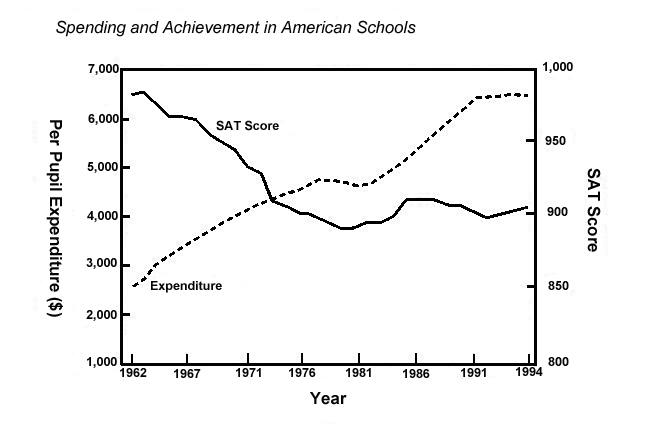
\includegraphics[width=\linewidth]{3}
\end{figure}
\begin{center}
	\textit{\footnotesize Sources: Educational Testing Service, U.S. Department of Education, Digest of Education Statistics 1994 (Washington: National Center for Education Statistics, 1994), Tables 127 and 165.\\	
	Note: SAT scores for 1961-67 are means for all students; subsequent scores are averages for college-bound seniors.}
\end{center}
\switchcolumn
\begin{figure}
	\centering
	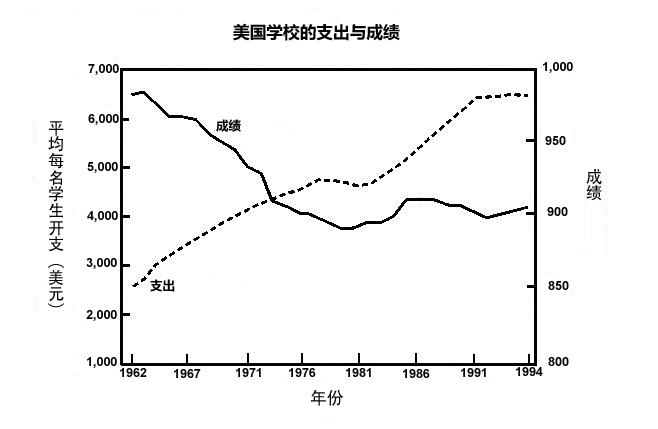
\includegraphics[width=\linewidth]{4}
\end{figure}
\begin{center}
	\textit{\footnotesize 引自:美国教育部教育考试服务中心1994年 《教育统计摘要》 (华盛顿:国家教育统计中心,1994),表 127和表165\\
	注释:1961 $\sim$ 1967年的成绩指所有学生;后面年份的成绩是指高中毕业班学平生平均成绩}
\end{center}
\switchcolumn*
Not only are test scores declining, but businesspeople complain that graduates of American high schools are not prepared
for work. American students tell survey researchers that their
reading, writing, and math skills are good, but employers have
a different view. In one survey, only 22 percent of employers
thought that recently hired high school graduates had sufficient math skills, and only 30 percent were satisfied with new
hires' reading abilities. When BellSouth tested technician applicants, only 8 percent passed. Motorola spends \$1,350 per
employee each year teaching basic skills. Many companies are
rewriting manuals to accommodate poor reading skills or de-
signing technology that doesn't require reading or math skills.
The schools are not turning out a workforce prepared for
global competition.
\switchcolumn
不仅考试分数下降,而且企业也在抱怨美国高中毕业生的
知识准备和能力根本无法胜任工作要求。美国学生告诉调查研
究者说他们的阅读、写作和数学能力是很不错的,但雇主们对
此有不同的看法。一项调查表明,只有 22\% 的雇主认为现在
的高中毕业生有足够的数学能力,只有30\% 的雇主对新雇员
的阅读能力表示满意。南方贝尔公司对申请技术员的应聘者进
行测试,结果只有8\%的人合格。摩托罗拉公司则每年在每位
员工身上花1350美元培训基本技能。很多公司都重新编写职
业手册,以适应员工那可怜的阅读能力,或者采用一些不需要
阅读和数学能力的技术。我们的学校并没有培养出足以应对全球化竞争的劳动力。
\switchcolumn*
Every form of communications and information transfer in
our society has been revolutionized in the past 20 years, yet the
schools still look the same way they did 200 years ago---a
teacher lecturing in front of thirty students, with the school day
and the school year geared to the rhythms of an agricultural society. We can only imagine the dynamic innovations in learning
that profit-seeking companies might have produced had they
been delivering education.
\switchcolumn
在美国,过去20年 ,所有的通信和信息传递方式都发生
了革命性的变化,然而学校看上去仍然像200年前没有区别
---一名老师在30名学生面前讲课,仍然严格按照农业社会
的节奏来安排学制。可以想像,富有活力的学习方式变革将由
追求利润的公司创造出来,并传给学校教育。
\switchcolumn*
Libertarians want to remove education from the bureaucratic
state and make it truly responsive to students and parents. Private schools do a much better job at educating students, but
most parents find it difficult to pay once for the public school
system and then pay again for private school. If they didn't
have to pay school taxes, they could afford to purchase education in the marketplace. Or if taxes were lower, more families
could afford to have one parent educate children at home.
\switchcolumn
古典自由主义者希望将教育从官僚机制下的国家手里拿
走,让教育真正对学生和家长负责。私立学校在教育学生方面
做得更好,但是很多家长发现,很难在为公立学校体系付过钱
之后再为私立学校付钱了。如果不必支付教育税,他们就有能
力在市场上购买教育了。如果税率低一些的话,就会有更多家
庭能够让一名家长专职在家教育子女。
\switchcolumn*
Many people fear that children wouldn't get educated if
schooling weren't free and compulsory. Historical evidence
shows that in England and the United States the vast majority
of children were educated before the government took over
schooling. Even Senator Edward M. Kennedy, no fan of civil society and the market process, has claimed that literacy was
higher before the advent of public education than it is today---
which makes one wonder why he wants to pour more and more
money into a government system that is delivering such poor
results.
\switchcolumn
很多人担心,如果学校教育不是免费和强制义务的话,孩
子们就得不到教育。历史证据显示,在政府接手学校教育之
前,英国和美国的大多数孩子都受到了教育。甚至爱德华$\cdot$肯
尼迪参议员 --- 他并不是市民社会和市场经济的爱好者 --- 也
说 ,公立教育建立之前的识字率比现在要高 --- 这让人很迷
惑,为什么他还主张把越来越多的钱投向政府的教育体系,这
个教育体系的产出是如此之少。
\switchcolumn*
For people who are sympathetic to these arguments but not
quite persuaded that a totally free market would supply enough
education, libertarians have offered some halfway steps toward
educational freedom. We could take the money we currently
spend on public school students---about \$6,800 per student
per year---and give it directly to families in the form of a scholarship or voucher, to be spent at the public or private school of
their choice. That way, education would still be funded by compulsory taxation but at least parents could choose the kind of
school they want for their child. Even better would be to expect
rich and middle-class families to pay for their own children's education---surely education should be considered a basic cost of
bringing up children---but supply a tax-funded voucher for
poor children. That would allow a significant reduction in
school taxes, which would enable most parents to pay for education on their own.
\switchcolumn
一些人赞同上述观点,但并不确信完全的自由市场可以提
供足够的教育。对这些人,古典自由主义者提供了通向教育自
由化的折中办法。把现在花在公立学校学生身上的钱 --- 每位
学生每年大约是6800美元 --- 以奖学金或者教育券的形式直
接交给家庭。人们可以自由选择把这笔钱用在公立或者私立学
校。这种办法,教育仍然是由强制性税收来支持,但是至少家
长们能够按照自己的意愿为孩子选择学校了。如果富人和中产
阶级家庭能够为自己孩子的教育付费,同时给穷人的孩子提供
由税收支持的教育券,那就更好了。教育本来就应当被看作抚
养孩子的起码成本。这种办法将让教育税大幅度削减,也会促
使大多数父母自己为孩子的教育付费。
\switchcolumn*
Like Soviet factories a few years ago, American schools today
are technologically backward, overstaffed, inflexible, unresponsive to consumer demand, and operated for the convenience of
top-level bureaucrats. We need to open up the \$300-billion-a-year education industry and let the market process in. Imagine
the ways schools competing for parents' dollars would find to
meet the needs of individual students. Educational technology
is in its infancy, but create a market and we'll see billions being
spent on research and development. We'll see schools that respect parents' values and welcome parents' involvement. We'll
learn, as one talented educator puts it, that ``we don't need to get kids ready for school, we need to get schools ready for kids.''
That's what happens in markets.
\switchcolumn
就像多年以前的苏联工厂一样,今天的美国学校技术落
后 ,机构臃肿,僵化,对消费者的需求不负责,内部运作方式
只是为了髙层官僚的方便。应当开放一年3000亿美元的教育
产业,引入市场机制。可以想像,学校在为家长们手里的钱而
竞争的时候,会努力寻找满足学生个人需要的方式。教育技术
仍然在婴儿期,但是只要创造一个市场,就会有数以十亿计的
美元被用到研究和发展之上。学校会尊重家长们的价值观,欢
迎家长们对教学过程的参与。正如一位天才的教育家指出的那
样,“孩子们不需要为学校做好准备,学校需要为孩子们做好准备。” 这正是自由教育市场会出现的现象。

\switchcolumn*[\section{Protecting Civil Liberties\\保护公民自由}]
As we've said before, libertarianism is the view that each person
has the right to live his life in any way he chooses so long as he
respects the equal rights of others. Thus libertarians oppose
government restrictions on individual behavior as long as one's
actions don't infringe on the rights of others. That doesn't necessarily mean approving or endorsing any particular behavior; it
just means that the coercive power of the state should be limited to protecting our rights. It would be impossible to make a
list of all the civil liberties we have; we tend to identify particular civil liberties as the state attempts to restrict them. The Bill
of Rights reflected the Founders' specific experience with
British restrictions on individual rights; but, recognizing that it
was impossible to enumerate all individual rights, they added
the Ninth Amendment---reserving to individuals other rights
not enumerated---and the Tenth Amendment---reiterating
that the federal government has only those powers set out in
the Constitution.
\switchcolumn
正如我们前面所谈到的那样,古典自由主义的观点是每个
人有权按照自己选择的方式来生活,同时尊重别人的同等权
利。因此,古典自由主义者反对政府在个人行为并没有侵犯别
人权利的情况下对其进行限制。这并不意味着赞成或支持任何
特定的行为;而只意味着强制权力或国家应当受到限制,以保
护我们的权利。要列举我们所拥有的公民自由是不可能的事
情 ;我们倾向于在国家试图限制某些权利时对特定的公民自由
进行甄别确认。《权利法案》反映了建国先贤们在英国限制个
人权利时的特定经验;但是,在认识到不可能列举所有个人权
利之后,建 国 先 贤 们 在 《美国宪法》 中加入了 “第九修正
案”  --- 其他未列举的权利保留给个人,以 及 “第十修正
案”  --- 重申联邦政府仅拥有宪法授予的权力。
\switchcolumn*
Civil libertarians often find themselves defending an individual's right to engage in actions that they may find reprehensible. As Hayek writes in \textit{The Constitution of Liberty}, ``Freedom
necessarily means that many things will be done which we do
not like.'' We all benefit from the general condition of freedom,
not just because it entitles us to do what we want, but because
civilization progresses through trial and error, through individuals' trying new ways of life. He goes on to say, ``The freedom
that will be used by only one man in a million may be more important to society and more beneficial to the majority than any
freedom that we all use.''
\switchcolumn
古典自由主义者发现自己常常在保卫个人做受非议之事的
权利,就像哈耶克在《自由宪章》一书中所说:“自由必然意
味着很多人会做我们不喜欢的事情。”’我们之所以会在普遍的
自由状态中受益,并不只是因为自由让我们想做的事情,而是
因为文明就是通过不断地试错,通过个人不断尝试新的生活方
式来取得进步的。他继续说:“百万人中仅有一人所能使用的
自由对社会的重要性以及对大多数人的助益,可能要超过人人
都可以使用的自由。”
\switchcolumn*
Civil society offers room for individuals to live in ways that
they choose, even if they may offend the majority. However, it
also affords people the opportunity to limit their own freedom
of action by entering into contracts and associations with others
and to use their property to create an environment they find congenial. For instance, people have a right to smoke tobacco or
marijuana even if the majority find smoking both dangerous
and disgusting. But other people have a right to forbid smoking
in their own homes, restaurants, or businesses. People have a
right to paint their houses purple, but not if they have voluntarily entered into an agreement with their neighbors---in a
housing development with restrictive covenants, for instance---
to paint their house only in pastel colors.
\switchcolumn
市民社会给个人提供了按照自己选择的方式生活的空间,
哪怕这种生活方式可能会遭到大多数人的反对。但是它也给人
们提供了机会,让人们可以通过与他人签订合同,或者通过加入、组成社会组织来限制他人的自由,目的是用财产创造出一种适合自己的环境。例如,即使大多数人认为吸烟既危险也令
人厌恶,人们也有权抽烟或者吸食大麻。但是人们有权在他们
自己家里、餐馆或者公司里禁止吸烟。人们有权把自己的房子
粉刷成紫色,但是如果已经自愿和邻居签订契约 --- 例如,在
有限制性条款的房屋开发过程中,规定只能把房子粉刷成浅色
的话,他们就不能这么做了。
\switchcolumn*
Libertarians defend the right of individuals to freedom of
speech, freedom of the press, and freedom of broadcast, even
though they may exercise that freedom in ways that offend others in society, whether through sexually explicit language, racist
magazines, or communist books. Every new technology brings
with it new demands for censorship, and electronic communication is no exception. Fortunately, the fabulously complex, international Internet will prove extremely difficult to censor, and
governments will be increasingly hard-pressed to limit what
their citizens can know.
\switchcolumn
古典自由主义者桿卫个人的言论自由、新闻出版自由、广
播自由,即使这些人行使自由的方式会触怒社会中的其他人,
也许是通过赤裸裸的性语言、种族主义杂志或者共产主义书
籍。每一种新技术的出现都会带来对其进行审查的要求,电子
通信技术也不例外。幸运的是,互联网的复杂程度和国际化使
得对它进行审查难度极高,但政府仍会不断加紧限制公民所能
得到的信息。
\switchcolumn*
Sexuality is another intimate aspect of life that governments
have meddled in from time immemorial. As recently as the
1960s, homosexual relations were illegal in almost all states,
and about twenty states still have such laws on the books as we
approach the twenty-first century. When these laws were vigorously enforced, they drove gay people underground and created
much misery. Once gay people stood up for their rights, governments began to back away from enforcing the laws. However, the Supreme Court ruled in 1986 that there was no
constitutional right to choose one's own consenting adult sexual partners, and sodomy laws are still used, for instance, to
deny gay parents custody of their children. Such laws should be
repealed, and all Americans should have equal rights.
\switchcolumn
性是个人的私事,而恰恰是这个领域被政府干预了数千
年。直 到 1960年代,同性恋几乎在美国所有的州都是非法的,
而目前,这样的法律仍然在大约20个州存在。当政府积极执
行这些法律的时候,同性恋就被迫转入地下,并且因此产生了
大量悲剧。而一旦同性恋者起来捍卫自己的权利,政府就开始
从执行法律的立场上逐渐后退。然而,最高法院在1986年宣
布,在双方同意的情况下选择自己的成年性伙伴并不是宪法权
利 ,鸡奸法仍然有效,否认同性恋父母有收养孩子的权利。这
样的法律应该废除。所有美国人都应当拥有同等的权利。
\switchcolumn*
In the name of protecting our safety, government restricts
our right to make our own decisions and assume responsibility
for the consequences of those decisions. Mandatory seatbelt and
helmet laws, for instance, deny us the right to choose the risks
we want to assume. The Food and Drug Administration denies
us the right to choose the vitamins, pharmaceutical drugs, and
medical devices that we want. Surely the decision to pursue a
particular course of medication is as personal and intimate as any choice could be. Many doctors believe that marijuana has
medical benefits, for relief of glaucoma and to reduce the pain
and nausea associated with AIDS, cancer, and chemotherapy;
those doctors may be right or wrong, but the decision should be
up to the patient, not a bureaucratic agency in Washington.
\switchcolumn
政府还以确保安全的名义,限制我们对自己的事务做决定
并对后果承担责任的权利。法律规定开车时必须系安全带,在
工地必须戴安全帽,这就剥夺了我们自愿选择承担风险的权
利。美国食品与药品管理局(FDA) 也剥夺了我们自愿选择维生素、药品和医疗服务的权利。毋庸置疑,选择药物和治疗
方式就像其他选择一样完全是个人的私事。很多医生都确信大
麻对缓解青光眼症状、减轻艾滋病、癌症和化疗引起的痛苦有
明显效果。这些医生可能是对的,也可能是错的,但是对此做
出决定的应该是患者,而不是华盛顿的官僚机构。
\switchcolumn*
One of the most disturbing trends in civil liberties is the increasing militarization of law enforcement in the United States,
much of it---though not all---an attempt to escalate the increasingly futile War on Drugs. Once again, the failure of one
government intervention leads to pressure for more intervention. Drug prohibition fails to stop the drug trade, so the government points to that very failure as a reason to hire more
police, pressure foreign governments, expand its powers of
search-and-seizure and civil forfeiture, deprive law-abiding people of public telephones in drug-trade areas, subject all employees to drug testing, and so on. There are now fifty-two federal
agencies whose officers have the power to carry firearms and
make arrests. Maybe that's why we've seen an increasing number of violent federal assaults on individual Americans, from the
deaths of Vicki and Sammy Weaver at Ruby Ridge, Idaho, to
the killing of Donald Scott in a trumped-up marijuana bust in
Malibu to the tanks-and-helicopter assault on the Branch Davidians in Waco, Texas, that left more than eighty people dead.
\switchcolumn
在美国,在公民自由这个问题上最让人不安的趋势之一
是 ,执行法律时越来越多地使用武力,其 中 很 多 武 力(当然
不是全部)的使用都使得本来已经缓解的反毒品战争不断升
级。又一次,政府干预的失败导致了更多的干预。禁毒并没有
阻止毒品贸易,而这种失败却让政府认为他们有理由雇用更多
警察、向外国政府施加压力、扩张搜查扣押和民事没收的权
力、剥夺毒品交易地区守法公民使用公用电话的权利、迫使所
有雇员进行毒品测试。现在有52个联邦机构有权持有武器并
且实施逮捕。这也许就是联邦官员侵犯美国公民个人权利的事
件不断增多的原因。从爱达荷州红宝石脊郡的维基$\cdot$维弗和山
姆 $\cdot$ 维弗被杀事件\footnote{民团主义(Vigilantism)大致起源于18世纪60年代,认为人民有拥有武器和革命的权利,他们要保卫美国立国之初那种乡村本位的自由价值,反对大政府式的联邦主义,也反对和平主义。民团主义理念之下,产 生 出 所 谓 “民兵组织”。兰迪$\cdot$维弗是美国爱达荷州红宝石脊郡的民兵组织领袖。由于各种民兵组织	日益活跃,美国政府于1992年起展开整肃。当年,联邦调查局围攻民兵领袖维弗在爱达荷州红宝石脊郡的住宅,韦弗的妻子维基$\cdot$维弗与儿子山姆$\cdot$维弗被杀。} ,到亿万富翁唐纳德$\cdot$斯科特在马里布市
因捏造的私藏大麻罪被警察杀害事件\footnote{唐纳德$\cdot$斯科特(Donald Scott),美国加州马里布市百万富翁,因被怀疑藏有大麻,1992年 10月 2 日在家中被突然闯人的洛杉矶司法局和其他5个执法部门的执法人员枪杀。},到大卫教派在德克萨斯州韦科的总部被坦克和直升机武装进攻,造成超过80人死亡的严重事件\footnote{大卫教派(Branch Davidians)是一个宣扬“世界末日” 的极端教派。1993年2月28日,美国联邦烟酒与军火管理局在掌握了大卫教派囤积大量武器的事实后,包围了骆驼山庄,试图拘捕教派头领考雷什。大卫教派进行武装抵抗,拘捕计划失败。联邦调查局接手此案,调来450名军警,数十辆装甲车、坦克和直升机,继续对庄园实施包围。双方对峙的51天中无一信徒投降。此后,联邦调査局用坦克和直升机进攻庄园。庄园起火,除 9 人外,包括考雷什在内的86人全部葬身火海。}。
\switchcolumn*
As Thomas Jefferson said, ``The price of liberty is eternal vigilance.'' Constitutions help to protect liberty, but only a society
of people determined to guard their freedom against encroachment can, over the long term, resist the natural tendency of
power to expand.
\switchcolumn
正如杰斐逊所说, “ 自由的代价就是永远保持警惕。”美
国宪法有助于保护自由,但是长期来说,只有全体社会成员决
心保卫他们的自由不受侵犯,才能抵抗政府权力天然扩张的
趋势。

\switchcolumn*[\section{Protecting the Environment\\保护环境}]
Environmental quality is an important aspect of a good society,
and many people are skeptical that the free market can supply
it adequately. While there is no perfect solution to environmental problems in any political or philosophical system, libertarianism offers the best available framework for producing the
environmental protection that people want.
\switchcolumn
环境质量是一个良好社会的重要组成部分。很多人对自由
市场能否充分提供这个产品表示怀疑。对环境问题,任何政治
制度和理论体系都没有完美的解决方案,而古典自由主义解决
环境问题的框架是其中最好的。
\switchcolumn*
Economic growth helps to produce environmental quality. Wealthier people and wealthier societies can afford to demand
and pay for better air and water quality. People struggling to
survive or to rise above backbreaking labor don't care very
much about environmental amenities; when people have
reached a comfortable standard of living, they turn their attention to such higher-order ``goods.'' In fact, air and water quality
in the United States has improved steadily during this century,
and our rising life expectancy is the best evidence that our environment is becoming more, not less, people-friendly.
\switchcolumn
经济增长有利于提髙环境质量。人们越富裕、社会越富
裕 ,就越有能力为更清洁的空气和水买单。在生存边缘和艰辛
劳动中挣扎的人们是不会关心环境是否优雅的;当人们达到舒
适的生活标准的时候,他们才会把注意力转移到这样更高要求
的 “产品” 上去。事实上在美国,空气和水的质量得到了持
续改善,预期寿命的提高就是环境变得越来越适宜于人类居住
的最好证明,而不是相反。
\switchcolumn*
As economies become more efficient and more technologically advanced, they use fewer resources to produce greater
value for consumers. Remember, the basic economic problem is
to get more value out of resources. Because soft-drink companies want to save money, they developed ways to use much less
tin---and later, aluminum---in each can. In 1974 a pound of
aluminum yielded 22.7 beverage cans; in 1994 the same pound
yielded 30.13 cans. The same profit incentive impels companies
to seek a use for their waste products; the Coca-Cola Company
discovered that the sheets of metal out of which they punched
bottle caps made ideal furnace filters. When Coca-Cola's
Minute Maid division makes orange juice, no part of the orange
goes to waste: the company squeezes out every drop of juice,
presses oil out of the peel, and feeds the rest to cows.
\switchcolumn
随着经济变得越来越有效率,技术越来越先进,整个经济体能够用更少的资源来为消费者产生更大的价值。不要忘了,
经济的最基本问题是如何以最少的资源获得最大的价值。由于
软饮料公司希望降低成本,他们想尽各种办法在制造每个饮料
罐的时候使用更少的铁皮(以及后来使用的铝皮)。1974年,
1磅铝能够制造22. 7 个饮料罐;而到了 1994年 ,1镑铝能够
制造30. 13个罐子。同样,对利润的追求驱使着各个公司对废
物废料进行充分利用;可口可乐公司发现压制瓶盖后剩下的废
金属板用来做锅炉滤网相当理想。可口可乐的美汁源部生产橙
汁的时候,不浪费橙子的任何部分:榨干每一滴橙汁,从橙子
皮当中把油压出来,然后把剩下的东西喂奶牛。
\switchcolumn*
One of the biggest generators of environmental problems is
what the environmentalist Garrett Hardin called ``the tragedy
of the commons.'' When resources---such as a common grazing
area, forest, or lake---are ``owned'' by everyone, they are effectively owned by no one. No one has an incentive to maintain
the value of the asset or use it on a sustainable basis. It's like six
kids sharing a milkshake: each one has an incentive to drain the
cup before the others do. When timber companies cut trees in a
national forest, their incentive is to cut them all, now, before
some other company gets a permit to use the same area. When
timber companies cut trees on their own land, they replant as
many as they cut, so they'll have a moneymaking asset for years
to come. One of the biggest environmental problems today is
the depletion of ocean fisheries, a clear example of the tragedy
of the commons for which a privatization solution is urgently
needed.
\switchcolumn
产生环境问题的最大发动机是环保主义者哈丁(Garrett
Hardin)所 说 的 “公地悲剧” (Tragedy  of the commons )。 当
资 源 “属于” 所有人的时候,如公共牧场、森林或湖泊,它
们就事实上不属于任何人。没有人有动机来维护财产的价值,
或者以可持续方式来使用这些财产。这就像六个小孩分牛奶:
每个人都想在别的孩子之前把牛奶喝光。如果木材公司在国家
森林砍伐木材,他们就希望在别的公司得到此区域的砍伐许可
之前把树木都砍光。如果木材公司在自己的土地上砍树,他们
砍掉多少就会重新种植多少,这样他们的财产才能在未来的年
份里继续产生财富。目前最大的环境问题之一是海洋鱼类因过
度捕捞而衰竭。这是公地悲剧最清晰的例子。要解决这个问
题 ,就需要尽快实施海洋渔场私有化。
\switchcolumn*
So how can a libertarian perspective help to improve environmental quality? First, a free society offers a diversity of approaches  to  solving  problems.  Competitive  systems---
capitalism, democracy, and science---allow ideas to be tested
and successful ideas to be emulated. Command-and-control
regulation from Washington cannot manage efficiently the environmental issues confronting hundreds of thousands of commercial enterprises any more than it can adequately guide a
society's economic activities.
\switchcolumn
那么古典自由主义如何帮助改善环境质量呢?首先,自由
社会提供了解决问题的各种路径。竞争的机制 --- 资本主义、
民主和科学 --- 可以让各种想法进行试验,并且允许对成功经
验进行模仿复制。而华盛顿那种命令与控制式的管制手段既然
不能有效地引导整个社会的经济活动,那么它在处理成千上万的商业公司面临的环境问题时也不可能更有效。
\switchcolumn*
Second, private owners take better care of resources than do
public owners. Private property rights mean that lines of authority are clear and that specific people will reap either the benefits
or the costs of their actions. The way to avoid the tragedy of the
commons is to privatize the commons. As environmental economist Richard Stroup says, property rights must be ``3-D'':
``clearly defined, easily defended against invasion, and divestible
(transferable) on terms agreeable to buyer and seller.'' Why are
buffalo an endangered species but not cows? Why did passenger
pigeons disappear but not chickens? Because owners have an incentive to maintain what they own. Congress should stop its annual politicized debates over how to manage federal lands---timber quotas, mineral rights, grazing fees, offshore drilling---and move toward privatization of natural resources so that private stewards can exercise proper stewardship.
\switchcolumn
其次,私人资源的所有人能够比公共资源的所有人更好地
照看好资源。私人财产权意味着权利范围清晰,有明确而具体
的人从财产中获得收益或者对其行为承担成本。避免公地悲剧
的办法就是公地私有化。正如环境经济学家斯特鲁普所说,财
产权必须有3 个维度:“界定清晰,易于防止侵犯,在买卖双
方同意的情况下易于转让。”为什么北美水牛是瀕危物种而奶
牛不是?为什么灭绝的是候鸽而不是鸡?因为财产所有者有足
够激励维护自己的财产。国会应当停止每年对如何管理联邦土
地问题的政治化争论,例如什么森林砍伐份额、采矿权、牧场
使用费、海上钻探之类,而应当讨论如何对自然资源进行私有
化,好让私人管理者对其进行恰当的管理。
\switchcolumn*
Third, environmental problems should be handled at the
most local level possible. Political activists on both sides of environmental issues have run to Washington to get their own
agenda imposed on the whole country. But the principles of federalism and subsidiarity would suggest that problems should be
handled privately if possible and, if not, then at the local or
state level before any federal involvement is considered. We lose
the benefits of decentralization and experimentation when we
impose one solution on the whole country.
\switchcolumn
第三,环境问题应当尽可能在最基层处理。在环境问题上
彼此对立的双方政治活动家常常跑到华盛顿,试图把自己的计
划在整个国家推行。但是根据联邦主义和自治优先原则\footnote{自治优先原则(Subsidiarity  principle),又译为辅助原则、附属原则、基层化原则、决策权从属于下原则。在这里译者按其本意译为“ 自治优先原则”。是联邦主义的基本原则之一,意思是把决策权尽量下放至地方或组织内较低级的部门。这个原则在企业管理当中也得到了广泛运用,也就是在企业中根据职责和有效完成原则,把事务决策权交给具有该权利的最低层。}, 问题应该首先尽可能在私人领域来解决,私人不能解决,则应当尽可能在地方或者州的层面解决,仍然不能解决的话,才应该
允许联邦政府介入。把一个解决方案应用到整个国家,会失去分散决策和试验的好处。
\switchcolumn*
Fourth, where markets don't always work---where property
rights are ill defined or goods are hard to divide---common law
is an important problem-solving institution. Anywhere people
live together, environmental problems will arise---smells, runoffs, factory smoke. As individuals take such disagreements to
court, they help to define property rights and the law. Such an evolving, decentralized production of law leads to better answers than a one-size-fits-all legislative command.
\switchcolumn
第四,在市场不能起作用的时候,即财产权很难界定或者
物品很难分割的时候,普通法是一种重要的解决问题机制。在
任何人类聚居的地方都会产生环境问题 --- 臭气、污水排放、工厂产生的烟雾等。当人们带着这些争执到法院的时候,这些
诉讼就有助于界定产权和规则(即法律)。这样一种演进的、
分散创制的法律比一刀切式的立法能够更好地解决问题。
\switchcolumn*
Fifth, the libertarian emphasis on individual responsibility
means that we should avoid the invitation to personal irresponsibility entailed by collective liability and adopt a ``polluter-pays'' approach to liability issues. Superfund is the classic
mistake here. All producers of hazardous waste are required to
pay into the fund, which is then allocated by a regulatory bureaucracy to clean up specific sites. We should hold individual
polluters responsible for damage they actually do, rather than
impose collective guilt on an entire industry and eliminate
every company's incentive to avoid pollution. The aim of environmental policy should be the protection of persons and their
property, as is true of our legal system generally.
\switchcolumn
第五,古典自由主义者强调个人责任,认为应当防止集体
负责所造成的个人不负责,在由谁承担责任的问题上采用
“谁污染谁付账” 的办法。“超级基金法”\footnote{超级基金法(Superfond),美国于1980年制定了《综合环境反应、赔偿与责任法》,通称《超级基金法》。该法创设了著名的“超级基金”,用于在无法确定责任主体或责任主体无力采取反应措施时,划出资金淸除污染。}就是一个典型的错误政策。这个法律要求所有产生危险废料的生产者都支付一笔
钱给超级基金,基金由一个管制机构来调配用来清理一些特定
地方的污染。我们应当让制造污染的人为他们实际造成的损害
负责,而不是为整个行业集体承担责任,因为这将让每家具体
的公司缺乏避免污染的动力。环境政策的目的应该是保护个人
和他们的财产,这是我们法律制度的总体目标。
\switchcolumn*
Finally, of course, smaller government means that government itself would stop polluting and encouraging environmental damage. Government environmental destruction was
rampant in the Soviet countries, but it is a real problem in
mixed economies as well. Government subsidies encourage the
clearing of tropical rain forests. Massive hydropower projects
from the United States to China are almost always government
sponsored. Farm programs, especially sugar quotas, have encouraged overuse of agricultural land. Governments without
such powers would do less damage to the environment as well
as to the economy.
\switchcolumn
最后,政府越小意味着政府本身将会停止污染,或者不再
助长对环境的破坏。政府破坏环境,这在前苏维埃国家是普遍
现象,在混合经济下这个问题也同样真实存在。政府的资助鼓
励了对热带雨林的开垦。从美国到中国的大型水利工程几乎都
是政府出资兴建的。农业计划尤其是糖的配额制度鼓励了过度
使用农业土地。政府如果没有这些权力的话,对环境的破坏就
会减少 --- 对经济也是如此。
\switchcolumn*
The institutions of private property, decentralized decision
making, common law, and strict liability will lead us to better
solutions---solutions that reflect the real costs and benefits of
environmental quality---than command-and-control regulation produced in a political process and implemented by regulators unaccountable for the consequences of their actions.
However, since both common law and property rights are constantly evolving, there are undoubtedly environmental issues
for which we do not yet have adequate solutions. We have developed property rights in water flows, in underground water
pools, in grazing land, in animal herds; but how can we develop
property rights in air? If global warming is a real problem---
and the evidence is still unclear on that point---could property
rights or common law lead us to a solution?
\switchcolumn
私人产权、分散决策、普通法和严格区分责任的制度在一
起所得出的解决方案 --- 反映了环境质量的真实成本和收益的
解决方案 --- 比通过政治程序产生,并由不必为自己行为承担
后果的管制官员所执行的命令控制式的管制要好得多。然而,无论是普通法还是财产权都还在不断演进过程中,毫无疑问,
对环境问题并没有完美的解决办法。已经能在流动水域、地下
水域、牧场、畜群中划分产权,但是怎样在空气中划分产权
呢?如果全球变暖是一个真问题的话 --- 其实证据仍然不足
--- 那么财产权和普通法能够引导我们找到解决办法吗?
\switchcolumn*
Economists, legal scholars, judges, businesspeople, and property owners are involved in an ongoing search for answers to
such questions. Free-market or at least market-oriented institutions that have developed recently to address environmental is-
sues rationally and at the least cost to society include pollution
charges, tradeable emission permits, markets for recyclable
trading, and performance standards (instead of regulations prescribing technologies and specific kinds of pollution reduction).
Those are not perfect libertarian solutions, and more work
needs to be done, but they are examples of how we can achieve
environmental quality without either politicizing the environment or imposing unnecessary costs on our economy.
\switchcolumn
经济学家、法律学者、法官、商人和财产所有者在不断探
索这些问题的答案。最近,为了理性解决环境问题,或者至少
让社会付出最小代价,人们发展出一些自由市场制度或者至少
是以市场为导向的制度,包括排污费、排污许可交易、可回收
垃圾交易市场以及环境绩效标准(不是对指定技术和特定种
类的污染排放进行管制)等。这些并不是完美的古典自由主
义解决方案,在这个问题上还有很多工作要做,但是这些例子
告诉我们,如何在不把环境问题政治化或者不给经济增加不必
要负担的情况下达到环境质量目标。
\switchcolumn*
A few years ago, at a scholarly conference on environmental
issues, I heard a professor of biology who had run a ranch in
Montana for twenty years discuss some of the many questions
he faced about how best to manage the resources on his ranch.
What struck me was that here was a man committed to environmental quality, professionally trained in biological science,
with decades of experience in resource management, and he
wasn't sure how to answer the questions that came up on his
own ranch. The lesson is that no one has all the answers, so no
one's answers should be imposed on the whole society. What we
need, as Karl Hess, Jr., wrote in Visions upon the Land, is ``a market of landscape visions, $\ldots$ a virtuous republic of independent,
caring, and responsible stewards'' of their own natural re-
sources.
\switchcolumn
几年前,在一个关于环境问题的学术会议上,我听一位在
蒙大拿州经营一家牧场二十年的生物学教授说到安排农场资源
时所面临的问题。让我印象深刻的是他这样一个人,致力于改
善环境质量,在生物学上受过专门训练,在资源管理领域有数
十年的经验,但即便如此,他也不知道如何解决自己的农场所
面临的问题。这个故事教育我们,没有任何人掌握所有的答
案 ,因此任何人的答案都不应该施加于整个社会。我们所需要
的是,如小卡尔$\cdot$ 海 丝 (Karl  Hess Jr.)\footnote{卡尔$\cdot$海 丝(Kari Hess, Jr. 1923$\sim$1994),美国政治理论家,古典自由主义和无政府资本主义的积极推动者。后来海丝因转向自由意志主义,与罗斯巴德积极合作,并参与了美国自由党的创建工作。} 在 《大地的景观》(\textit{Visions upon the Land}) 一书中所说: “一个自然景观的市场……一个对属于自己的自然资源进行独立、细心管理并承担责
任的管理者的共和国。”

\switchcolumn*[\section{Preserving Peace\\维护和平}]
The classical liberals always regarded war as the greatest
scourge that government could visit upon society. They abhorred the killing that war entailed, and they understood something else as well: war destroyed families, businesses, and civil
society. Preventing kings from putting their subjects at risk in
unnecessary wars was one of their major goals. Adam Smith
argued that little else was needed to create a happy and prosperous society but ``peace, easy taxes, and a tolerable administration of justice.''
\switchcolumn
传统的自由主义者常常把战争看作政府带给社会的最大灾
祸。他们憎恶战争带来的杀戮,他们也很清楚战争会毁灭家
庭 、商业和市民社会。阻止国王们把臣民陷入不必要的战争就
成了他们的主要目标之一。亚 当 $\cdot$ 斯密指出,要创造一个幸福
和繁荣的社会,除了 “和平、低税和过得去的司法”之外就
几乎不再需要别的什么了。
\switchcolumn*
The American Founders, happy to be free of the endless European wars, made peace and neutrality a cardinal principle of
the new government. In his Farewell Address, George Washington told the nation, ``The great rule in conduct for us, in regard to foreign nations, is in extending our commercial
relations to have with them as little political connection as possible.'' And Thomas Jefferson described American foreign pol-
icy in his First Inaugural Address this way: ``Peace, commerce,
and honest friendship with all nations---entangling alliances
with none.''
\switchcolumn
建国之父们非常庆幸美国人能够摆脱欧洲无休止的战争,
他们把和平和中立作为新政府的一项基本原则。乔 治 $\cdot$华盛顿
在其卸任演说中告诫人民:“关于与外国的关系,指导我们的原
则是尽可能扩展与他们的贸易关系,尽量减少与他们的政治联
系。” .杰斐逊在他的就职演说中这样描述美国的外交政策:“与
所有国家发展和平、贸易与诚实的友谊,不和任何国家结盟。”
\switchcolumn*
In the twentieth century, however, many people came to believe that the United States had to become involved in world
affairs and foreign wars. For fifty years U.S. foreign policy was
directed at defeating two totalitarian powers, Nazi Germany
and Soviet Russia. Today that great crusade is complete; America is secure, and no aggressive ideology threatens U.S. citizens
or world peace. But the huge diplomatic and military establishment that grew up during World War II and the cold war
refuses to declare victory and return to peacetime status. Instead, the American military remains large and expensive, and
American citizens are told that the post---cold-war world is
even more dangerous and unstable than the world that was
threatened by the Soviet Union. Thus we still have substantial
numbers of U.S. troops in Europe, Japan, Korea, and the Middle East.
\switchcolumn
然而,20世纪,很多人开始相信美国必须介入世界事务
和国外战争。在 50年中,美国外交政策的目标是打败两个极
权政权:纳粹德国和苏联。而今天伟大的十字军圣战已经结束
了。美国安全了。不再有激进的意识形态威胁美国公民或者世
界和平了。但在第二次世界大战和冷战中建立起来的庞大的外
交和军事体系拒绝宣告胜利,拒绝回到和平时期的状态。相
反 ,美国仍然保持着庞大和昂贵的军事力量。他们告诉美国公
民,后冷战时代的世界比苏联威胁之下的世界更加危险和不稳
定。因此仍然需要在欧洲、日本、韩国和中东保留相当数量的
美国军队。
\switchcolumn*
In just the few short years since the Persian Gulf War, we
have sent American troops, or been urged to send troops, to Somalia, Haiti, Bosnia, Liberia, Rwanda, Burundi, Macedonia,
and a host of other places. These places have just one thing in
common: no vital American interest is at risk there. Less than a
generation after the disaster in Vietnam, we seem to have forgotten the lessons of our intervention there. That intervention,
too, started small, with good intentions; no one expected that
we would end up with 500,000 American troops there and
55,000 American deaths.
\switchcolumn
就在海湾战争前短短的几年当中,美 国 派 遣 军 队 (或者
被迫派遣军队)到索马里、海地、波斯尼亚、利比里亚、卢
旺达、布隆迪、马其顿以及其他的地方。这些地方的共同点只
有一个:在那里美国利益没有受到任何威胁。在越战的灾难结
束后不到一代人的时间里,我们似乎已经忘记了在越南进行干
预的教训。那次干预开始时规模也很小,目的也很正当;没人
预料到最终会有50万军队陷在那里,也没人预料到,会有
55000名美国人死在那里。
\switchcolumn*
We need to remember a few simple rules about war and foreign policy. First, war kills people. Especially in the modern
world, it often kills as many civilians as soldiers. War cannot be
avoided at all costs, but it should be avoided wherever possible. Proposals to involve the United States---or any government---
in foreign conflict should be treated with great skepticism.
\switchcolumn
关于战争和外交,应当记住一些简单的法则。第一,战争
会死人。尤其是现代,战争中平民的死亡.会和士兵一样多。或
许 ,战争是无法避免的,但是应当尽可能避免战争。人们对所
有要求美国(或者任何政府)介入国外冲突的议案都应当持
最大的怀疑态度。
\switchcolumn*
Second, as discussed earlier, war creates big government.
Throughout history, it has provided an excuse for governments
to arrogate money and power to themselves and to regiment society. During World Wars I and II the United States government assumed powers it could never have acquired in
peacetime, powers such as wage-and-price controls, rationing,
close control of labor and production, and astronomical tax
rates. Constitutional restrictions on federal power were swiftly
eroded. That doesn't mean those wars shouldn't have been
fought. It \textit{does} mean that we should understand the consequences of war for our entire social order and thus go to war
only when absolutely necessary.
\switchcolumn
第二,正如前面所讨论的,战争产生大政府。在整个历史
中,每一次战争都成了政府攫取财富和权力以及把整个社会组
织起来的借口。第一次世界大战和第二次世界大战中,美国政
府获得了和平时期根本不可能得到的权力:工资和价格管制、
定量配给、直接控制劳动力和生产以及天文数字般的税收。对
联邦权力的宪法限制很快被侵蚀。不是说这些战争不应该打。
而是说我们\textbf{应该}了解战争对整个社会秩序所带来的后果,从而
只是在万不得已的时候才选择战争。
\switchcolumn*
Third, the United States can no more police and plan the
whole world than it can plan a national economy. Without a superpower threat to rally against, the politico-military establishment wants us to deploy our military resources on behalf of
democracy and self-determination around the world and
against such vague or decentralized threats as terrorism, drugs,
and environmental destruction. The military is designed to
fight wars in defense of American liberty and sovereignty; it is
not well equipped to be policeman and social worker to the
world.
\switchcolumn
第三,美国担任世界警察和对整个世界进行计划的能力不
可能超过它计划一个国家的经济的能力。在没有一个超级大国
威胁需要抵御的情况下,我们的政治军事系统想以民主与自决
的名义在世界范围内派遣军队,与恐怖主义、毒品和环境破坏
这些不确定和分散的威胁作战。美国军事力量是为通过作战来
保卫美国人民的自由和主权而设计的,并不是用来做世界警察和世界义工的。
\switchcolumn*
Fourth, our cold-war allies have recovered from the destruction of World War II and are fully capable of defending them-
selves. Not only is there no longer a Soviet threat to Europe, the
countries of the European Union have a collective population of
more than 370 million, a gross domestic product of \$7 trillion a
year, and more than 2 million troops. They can defend Europe
and deal with such problems as Serb aggression without U.S.
assistance. South Korea has twice the population and eighteen
times the economic output of North Korea; it doesn't need our
37,000 troops to protect itself.
\switchcolumn
第四,美国的盟国已经从第二次世界大战的破坏当中恢复
过来,并且完全具备保卫自己国家的能力。不仅苏联对欧洲的
威胁已经不复存在,而且欧盟国家也已拥有超过3. 7 亿的人
口,每年国民生产总值达到7 万亿美元,拥有超过200万人的
军队。他们有能力在没有美国帮助的情况下保卫欧洲,有能力
处理诸如塞尔维亚的侵略之类的问题。韩国的人口是朝鲜的2
倍 ,经济总量是朝鲜的18倍 ;它也并不需要3 .7 万美军来
保护。
\switchcolumn*
Fifth, the communications explosion means that the information imbalance between political leaders and citizens is much
reduced. Presidents often watch world events unfolding on
CNN, along with all the rest of us. That means that presidents
will find it more difficult to expect public deference on matters of foreign policy, so they should proceed cautiously in undertaking foreign commitments without popular support.
\switchcolumn
第五,信息爆炸意味着政治领导人和公民之间的信息不平
衡大大减少了。美国总统常常像其他人一样通过打开电视看
CNN来了解世界大事。这意味着,总统希望公众听从他的外
交政策就变得越来越困难了,因此,在没有民众支持的情况
下,总统采取对外行动会更加小心翼翼。
\switchcolumn*
The world is still full of potential threats, and the first purpose of government is to protect the rights of citizens. We must
maintain an adequate national defense, but we can defend the
vital interests of the United States with a military about half the
size of the one we have---especially if we reorient our foreign
policy to one of strategic independence, not global commitments to collective security agreements. That would still give
us about a million active-duty personnel. While we can eliminate some expensive cold-war weaponry designed to project
U.S. power far from our shores, we should pursue the possibility
of actually \textit{defending} U.S. citizens with an antiballistic-missile
defense system.
\switchcolumn
这世界仍然充满着潜在的威胁,而政府的首要责任是保护
公民的权利。必须维持足够的国防力量,但是我们能够以现在
大约一半规模的军事力量来保卫美国的重大利益 --- 尤其是把
外交政策调整为谋求战略性自主,而不是谋求全球范围内集体
安全体系时更是如此。我们仍然会拥有大约100万现役军人的
军事力量。与此同时,可以销毁一些冷战时期的昂贵武器,这
些武器是为了在远离海岸的遥远地方投放美国军事力量而设计
的。应当建立的是能真正\textbf{保卫}美国公民安全的反弹道导弹防御
系统。
\switchcolumn*
Libertarians who propose to bring U.S. troops home and concentrate on the defense of the United States are sometimes accused of being  ``isolationist.''  That's  a misconception.
Libertarians are in fact \textit{cosmopolitans}. We look forward to a world
bound together by free trade, global communications, and cultural exchange. We believe that military intervention around
the world hampers that effort. We also believe that, although
the world is growing closer together in many ways, it is inappropriate to view the whole world as a village in which everyone
must pitch in to stop every fight. In a dangerous world, with
terrorism and nuclear weapons, it is better to keep military conflicts limited and regional rather than to escalate them through
superpower involvement.
\switchcolumn
古典自由主义者提出的撤回美国军队、把军事力量集中于
保卫美国本土的建议,常常被批评为“孤立主义”。其实这是
一种误解。古典自由主义者是事实上的\textbf{世界主义者}。我们在寻
求建立一个由自由贸易、全球化和文化交流而结合在一起的世界。我们相信世界范围内的军事干预阻碍了这种努力。我们还
相信,尽管这个世界在很多方面结合得越来越紧密,但是把整
个世界看成一个村庄、每个人都必须积极阻止每一次冲突是不
恰当的。在一个存在恐怖主义和核武器的危险世界里,让军事
冲突保持一定限度和局限在地方冲突的范围,比通过超级大国
的干预而升级要好得多。
\switchcolumn*
What may seem to many readers an exhaustive review of
contemporary policy issues has hardly scratched the surface of
policy analysis, and many questions obviously remain unanswered here. The framework for libertarian policy analysis,
however, should be clear: individual liberty, private property,
free markets, and limited government create a vibrant and dynamic civil society that best accommodates the needs and preferences of millions of individual citizens.
\switchcolumn
也许对很多读者来说,我们对当代政策问题的回顾也已经
很详尽了,但其实这仅仅触及了这些政策分析的皮毛。很多问
题显然在这里并没有得到回答。但是古典自由主义政策的分析
框架应该已经很清楚了:个人自由、私人财产权、自由市场和
有限政府能够产生一个生机勃勃的富有活力的市民社会,最好
地满足数以百万计的公民个人的需求和偏好。

\end{paracol}